\documentclass[a4paper,11pt,twoside]{memoir}
\chapterstyle{veelo}

\usepackage{TUINFDA}

\usepackage{hyperref}					% links in pdf
\usepackage{cleveref}
\usepackage{graphicx}            			% Figures
\usepackage{verbatim}            			% Code-Environment
\usepackage[lined,linesnumbered,algochapter]{algorithm2e} % Algorithm-Environment

\usepackage{url}
\urlstyle{same}  % important for automatic line breaking in URLs

\usepackage{rotating}
\usepackage{lscape} % for rotating tables
\usepackage{lipsum}
\let\ab\allowbreak

\usepackage{pgf}					
\usepackage{tikz}					% tikz graphics
\usetikzlibrary{arrows,automata}

\usepackage{ngerman}
\usepackage[ngerman]{babel}
\usepackage{bibgerm,cite}       % Deutsche Bezeichnungen, Automatisches Zusammenfassen von Literaturstellen
\usepackage[ngerman]{varioref}  % Querverweise
% to use the german charset include cp850 for MS-DOS, ansinew for Windows and latin1 for Linux.
% \usepackage[latin1]{inputenc}

\thesistitle{Kosteneffizientes Ressourcenmanagement in verteilten Cloud Datenzentren}{Cost aware resource management in distributed cloud data centers}
\thesissubtitle{} % optional
\thesisdate{28.07.2015}

% all titles and designations have to be gender-related!
\thesisdegree{Diplom-Ingenieur}{Master of Science}
\thesiscurriculum{Informatik}{Computer Science} % your study
\thesisverfassung{Verfasser} % Verfasser
\thesisauthor{Andreas Egger} % your name
\thesisauthoraddress{Ospelgasse 35/3, 1200 Wien} % your address
\thesismatrikelno{0626885} % your registration number

\thesisbetreins{Priv.-Doz. Dr. Ivona Brandić}
\thesisbetrzwei{MSc. Dražen Lučanin}
\thesisbetrdrei{} % optional

% define page numbering styles
\makepagestyle{numberCorner}
\makeevenfoot{numberCorner}{\thepage}{}{}
\makeoddfoot{numberCorner}{}{}{\thepage}

% define custom macros for specific formats or names
\newcommand{\uml}[1]{\texttt{#1}}
\newcommand{\cd}{\textsf{Class Diagram}}

\begin{document}

\captionnamefont{\bfseries}

%%%%%%%%%%%%%%%%%%%%%%%%%%%%%%%%%%%%%%%%%
%%%   FRONTMATTER    %%%%%%%%%%%%%%%%%%%%
%%%%%%%%%%%%%%%%%%%%%%%%%%%%%%%%%%%%%%%%%
\frontmatter
\pagenumbering{roman}

%%%%%%%%%%%%%%%%%%%%%%%%%%%%%%%%%%%%%%%%%
%%%   TITLEPAGES    %%%%%%%%%%%%%%%%%%%%%
%%%%%%%%%%%%%%%%%%%%%%%%%%%%%%%%%%%%%%%%%

% the german title page is required as first page
% $Id: titlepage.tex 1752 2010-03-20 11:07:02Z tkren $
%
% TU Wien - Faculty of Informatics
% thesis titlepage
%
% This titlepage is using the geometry package, see
% <http://www.ctan.org/macros/latex/contrib/geometry/geometry.pdf>
%
% For questions and comments send an email to
% Thomas Krennwallner <tkren@kr.tuwien.ac.at>
% or to Petra Brosch <brosch@big.tuwien.ac.at>
%

\selectlanguage{ngerman}

% setup page dimensions for titlepage
\newgeometry{left=2.4cm,right=2.4cm,bottom=2.5cm,top=2cm}

% force baselineskip and parindent
\newlength{\tmpbaselineskip}
\setlength{\tmpbaselineskip}{\baselineskip}
\setlength{\baselineskip}{13.6pt}
\newlength{\tmpparindent}
\setlength{\tmpparindent}{\parindent}
\setlength{\parindent}{17pt}

% first titlepage
\thispagestyle{tuinftitlepage}

%
% Kludge: for each titlepage set \pagenumbering to a different
% style. This is used to fix a problem with hyperref, because there
% are multiple "page 1" and hyperref hates that
%
\pagenumbering{Alph}

\begin{center}
{\ \vspace{3.4cm}}

\begin{minipage}[t][2.8cm][s]{\textwidth}%
\centering
\thesistitlefontHUGE\sffamily\bfseries\tuinfthesistitle\\
\bigskip
{\thesistitlefonthuge\sffamily\bfseries\tuinfthesissubtitle}
\end{minipage}

\vspace{1.3cm}

{\thesistitlefontLARGE\sffamily \tuinfthesistype}

\vspace{6mm}

{\thesistitlefontlarge\sffamily zur Erlangung des akademischen Grades}

\vspace{6mm}

{\thesistitlefontLARGE\sffamily\bfseries \tuinfthesisdegree}

\vspace{6mm}

{\thesistitlefontlarge\sffamily im Rahmen des Studiums}

\vspace{6mm}

{\thesistitlefontLarge\sffamily\bfseries \tuinfthesiscurriculum}

\vspace{6.5mm}

{\thesistitlefontlarge\sffamily eingereicht von}

\vspace{6mm}

{\thesistitlefontLarge\sffamily\bfseries \tuinfthesisauthor}

\vspace{1.5mm}

{\thesistitlefontlarge\sffamily Matrikelnummer \tuinfthesismatrikelno} 

\vspace{1.4cm}

\vspace{0pt}\raggedright\thesistitlefontnormalsize\sffamily
\begin{minipage}[t][1.6cm][t]{\textwidth}%
  %
  an der

  Fakult\"{a}t f\"{u}r Informatik der Technischen Universit\"{a}t Wien
\end{minipage}

\begin{minipage}[t][4cm][t]{\textwidth}%
  \vspace{0pt}\raggedright\thesistitlefontnormalsize\sffamily
  %
  \begin{tabbing}%
	    \hspace{19mm} \= \hspace{66mm} \kill
	    \tuinfthesisbetreuung: \> \tuinfthesisbetreins\\
	    Mitwirkung: \> \tuinfthesisbetrzwei\\
	                \> \tuinfthesisbetrdrei
  \end{tabbing}
\end{minipage}

\begin{minipage}[t][1.5cm][t]{\textwidth}%
  \vspace{0pt}\sffamily\thesistitlefontnormalsize
  \begin{tabbing}%
    \hspace{45mm} \= \hspace{63mm} \= \hspace{51mm} \kill
    Wien, \tuinfthesisdate \> {\raggedright\rule{51mm}{0.5pt}} \> {\raggedright\rule{51mm}{0.5pt}} \\
    \> \begin{minipage}[t][0.5cm][t]{51mm}\centering (Unterschrift \tuinfthesisverfassung)\end{minipage}
    \> \begin{minipage}[t][0.5cm][t]{51mm}\centering (Unterschrift \tuinfthesisbetreuung)\end{minipage}
    \end{tabbing}
\end{minipage}

\end{center}

% we want an empty page right after first titlepage
\pagestyle{empty}
\cleardoublepage

% we're done with the titlepages, proceed with default pagenumbering
\pagenumbering{roman}

% restore baselineskip
\setlength{\baselineskip}{\tmpbaselineskip}
\setlength{\parindent}{\tmpparindent}

% back to normal geometry
\restoregeometry

\selectlanguage{english}

%%% Local Variables:
%%% TeX-PDF-mode: t
%%% TeX-debug-bad-boxes: t
%%% TeX-parse-self: t
%%% TeX-auto-save: t
%%% reftex-plug-into-AUCTeX: t
%%% End:


% an english translation may follow
% $Id: titlepage.tex 1752 2010-03-20 11:07:02Z tkren $
%
% TU Wien - Faculty of Informatics
% thesis titlepage
%
% This titlepage is using the geometry package, see
% <http://www.ctan.org/macros/latex/contrib/geometry/geometry.pdf>
%
% For questions and comments send an email to
% Thomas Krennwallner <tkren@kr.tuwien.ac.at>
% or to Petra Brosch <brosch@big.tuwien.ac.at>
%

% setup page dimensions for titlepage
\newgeometry{left=2.4cm,right=2.4cm,bottom=2.5cm,top=2cm}

% force baselineskip and parindent
%\newlength{\tmpbaselineskip}
%\setlength{\tmpbaselineskip}{\baselineskip}
%\setlength{\baselineskip}{13.6pt}
%\newlength{\tmpparindent}
%\setlength{\tmpparindent}{\parindent}
%\setlength{\parindent}{17pt}

% first titlepage
\thispagestyle{tuinftitlepage}

%
% Kludge: for each titlepage set \pagenumbering to a different
% style. This is used to fix a problem with hyperref, because there
% are multiple "page 1" and hyperref hates that
%
\pagenumbering{Roman}

\begin{center}
{\ \vspace{3.4cm}}

\begin{minipage}[t][2.8cm][s]{\textwidth}%
\centering
\thesistitlefontHUGE\sffamily\bfseries\tuinfthesistitle\\
\bigskip
{\thesistitlefonthuge\sffamily\bfseries\tuinfthesissubtitle}
\end{minipage}

\vspace{1.3cm}

{\thesistitlefontLARGE\sffamily \tuinfthesistypeen}

\vspace{6mm}

{\thesistitlefontlarge\sffamily submitted in partial fulfillment of the requirements for the degree of}

\vspace{6mm}

{\thesistitlefontLARGE\sffamily\bfseries \tuinfthesisdegreeen}

\vspace{6mm}

{\thesistitlefontlarge\sffamily in}

\vspace{6mm}

{\thesistitlefontLarge\sffamily\bfseries \tuinfthesiscurriculumen}

\vspace{6.5mm}

{\thesistitlefontlarge\sffamily by}

\vspace{6mm}

{\thesistitlefontLarge\sffamily\bfseries \tuinfthesisauthor}

\vspace{1.5mm}

{\thesistitlefontlarge\sffamily Registration Number \tuinfthesismatrikelno} 

\vspace{1.4cm}

\begin{minipage}[t][1.6cm][t]{\textwidth}%
  \vspace{0pt}\raggedright\thesistitlefontnormalsize\sffamily
  %
  to the Faculty of Informatics 

  at the Vienna University of Technology
\end{minipage}

\vspace{0pt}\raggedright\thesistitlefontnormalsize\sffamily
\begin{minipage}[t][4cm][t]{\textwidth}%
  \begin{tabbing}%
	    \hspace{19mm} \= \hspace{66mm} \kill
	    Advisor: \> \tuinfthesisbetreins\\
	    Assistance: \> \tuinfthesisbetrzwei\\
	                \> \tuinfthesisbetrdrei
     \end{tabbing}
\end{minipage}

\begin{minipage}[t][1.5cm][t]{\textwidth}%
  \vspace{0pt}\sffamily\thesistitlefontnormalsize
  \begin{tabbing}%
    \hspace{45mm} \= \hspace{63mm} \= \hspace{51mm} \kill
    Vienna, \tuinfthesisdate \> {\raggedright\rule{51mm}{0.5pt}} \> {\raggedright\rule{51mm}{0.5pt}} \\
    \> \begin{minipage}[t][0.5cm][t]{51mm}\centering (Signature of Author)\end{minipage}
    \> \begin{minipage}[t][0.5cm][t]{51mm}\centering (Signature of Advisor)\end{minipage}
    \end{tabbing}
\end{minipage}

\end{center}

% we want an empty page right after first titlepage
\pagestyle{empty}
\cleardoublepage

% we're done with the titlepages, proceed with default pagenumbering
\pagenumbering{roman}

% restore baselineskip
\setlength{\baselineskip}{\tmpbaselineskip}
\setlength{\parindent}{\tmpparindent}

% back to normal geometry
\restoregeometry


%%% Local Variables:
%%% TeX-PDF-mode: t
%%% TeX-debug-bad-boxes: t
%%% TeX-parse-self: t
%%% TeX-auto-save: t
%%% reftex-plug-into-AUCTeX: t
%%% End:
 % optional

%%%%%%%%%%%%%%%%%%%%%%%%%%%%%%%%%%%%%%%%%
%%%   ERKLAERUNG DER SELBSTAENDIGKEIT   %
%%%%%%%%%%%%%%%%%%%%%%%%%%%%%%%%%%%%%%%%%
\cleardoublepage
\selectlanguage{ngerman}
\chapter*{Erklärung zur Verfassung der Arbeit}

\tuinfthesisauthor\\
\tuinfthesisauthoraddress

\vspace*{1.2cm}

Hiermit erkläre ich, dass ich diese Arbeit selbständig verfasst habe, 
dass ich die verwendeten Quellen und Hilfsmittel vollständig angegeben 
habe und dass ich die Stellen der Arbeit - einschließlich Tabellen, 
Karten und Abbildungen -, die anderen Werken oder dem Internet im 
Wortlaut oder dem Sinn nach entnommen sind, auf jeden Fall unter Angabe 
der Quelle als Entlehnung kenntlich gemacht habe.\\

\vspace*{2cm}
\begin{tabbing}%
    \hspace{58mm} \= \hspace{28mm} \= \hspace{58mm} \kill
    {\raggedright\rule{58mm}{0.5pt}} \> \> {\raggedright\rule{58mm}{0.5pt}} \\
    \begin{minipage}[t][0.5cm][t]{58mm}
	\vspace{0pt}\sffamily\thesistitlefontnormalsize
	\centering (Ort, Datum)
    \end{minipage}
    \> \>
    \begin{minipage}[t][0.5cm][t]{58mm}
	\vspace{0pt}\sffamily\thesistitlefontnormalsize
	\centering (Unterschrift \tuinfthesisverfassung)
    \end{minipage}
\end{tabbing}


\selectlanguage{english}

%%%%%%%%%%%%%%%%%%%%%%%%%%%%%%%%%%%%%%%%%
%%%   ACKNOWLEDGEMENTS    %%%%%%%%%%%%%%%
%%%%%%%%%%%%%%%%%%%%%%%%%%%%%%%%%%%%%%%%%

% optional acknowledgements may be included in german or in english
%\chapter*{Danksagung}

Hier fügen Sie optional eine Danksagung ein.
 		% optional
\chapter*{Acknowledgements}

Optional acknowledgements may be inserted here.	% optional

%%%%%%%%%%%%%%%%%%%%%%%%%%%%%%%%%%%%%%%%%
%%%   ABSTARCT    %%%%%%%%%%%%%%%%%%%%%%%
%%%%%%%%%%%%%%%%%%%%%%%%%%%%%%%%%%%%%%%%%

\chapter*{Abstract}

Cloud computing services experienced increasing popularity over the recent years which caused the power demand of data centers to increase significantly. 
As energy costs represent a significant part of the total cost of data centers energy cost reductions in cloud computing environments play an important role for cloud providers to remain competitive and provide affordable cloud services. This thesis introduces a cloud framework to evaluate energy cost reductions in multi electricity market environments. It is shown that substantial cost savings are possible using intelligent resource scheduling algorithms with integration of energy price forecasts. 

This thesis consists of two parts. In the first part different forecasting models are evaluated to assess the performance of the models for energy price time series of different energy markets. A forecast simulation framework is introduced capable of dynamically managing energy price data from different power markets and generating forecasts based on that data. The framework incorporates methods for automatic model generation and evaluation as a basis for extended forecast simulations. 
A large scale forecast evaluation is conducted to gain insights into model accuracy across a wide range of energy price data. Different training periods, forecast horizons and energy price datasets lead to a comprehensive evaluation of the forecasting models. 

The second part is dedicated to large scale cloud simulations comprising different cloud schedulers and scenarios. An existing cloud simulation framework has been extended to perform simulations across a wide range of energy price data where different scheduling mechanisms have been introduced. 
A utility function has been defined for sophisticated evaluation of different criteria to decide on the best suitable VMs to migrate at any point in time. Criteria involve probability of SLA penalties and maximum cost benefits to appropriately handle the tradeoff between minimizing costs and providing an adequate level of quality of service. 

Results show that significant cost savings are possible with schedulers incorporating different criteria and energy price forecasts revealing promising results. Based on the defined cloud settings it illustrates the applicability of the proposed approach to real world scenarios of geo-distributed data centers connected to energy markets. 



\cleardoublepage
\selectlanguage{ngerman}
\chapter*{Kurzfassung}

Hier fügen Sie die Kurzfassung auf Deutsch gemäß den Vorgaben der Fakultät ein.

\selectlanguage{english}

%%%%%%%%%%%%%%%%%%%%%%%%%%%%%%%%%%%%%%%%%
%%%   CONTENTS    %%%%%%%%%%%%%%%%%%%%%%%
%%%%%%%%%%%%%%%%%%%%%%%%%%%%%%%%%%%%%%%%%
% uncomment to set document language to german (results in "Inhaltsverzeichnis", "Kapitel", "Abbildung", etc. instead of "Contents", "Chapter", and "Figure"), otherwise the document's language is english
%\selectlanguage{ngerman}

\setcounter{tocdepth}{1}

\cleardoublepage
\pagestyle{numberCorner}
\tableofcontents*

%%%%%%%%%%%%%%%%%%%%%%%%%%%%%%%%%%%%%%%%%
%%%   MAINMATTER    %%%%%%%%%%%%%%%%%%%%%
%%%%%%%%%%%%%%%%%%%%%%%%%%%%%%%%%%%%%%%%%

\mainmatter
\pagenumbering{arabic}
\pagestyle{numberCorner}


%%%%%%%%%%%%%%%%%%%%%%%%%%%%%%%%%%%%%%%%%
% 		 	Definition of remarks 					%
%																				%
% [c] - insert citation									%
% [r] - remove/replace prev. statement 	%
% [g] - insert graphic									%
%																				%
%%%%%%%%%%%%%%%%%%%%%%%%%%%%%%%%%%%%%%%%%


%%%%%%%%%%%%%%%%%%%%%%%%%%%%%%%%%%%%%%%%%
\chapter{Introduction}
\label{ch:intro}
%%%%%%%%%%%%%%%%%%%%%%%%%%%%%%%%%%%%%%%%%



\section{Motivation}

In times of cloud computing where computer resources are expected to be readily available from anywhere \cite{buyya2009cloud} and with an ever growing global network of interconnected devices cloud providers need to cope with increasing energy consumption in data centers as requests need to be handled at a rapid pace. 
As energy consumption is directly mapped to energy costs, cloud providers aim to reduce power consumption and thus electricity costs within data centers. 

Studies show that electricity costs for cloud systems comprising several large scale data centers is in the range of tens of millions of dollars per year \cite{qureshi2009cutting}. Energy consumption, related energy costs and high energy prices may slow down or hinder advancements in cloud computing. Thus, cloud providers must ensure that delivering their services remains profitable. Lower energy costs increase the competitive ability of cloud providers and bigger investments are possible. Likewise customers may benefit from more affordable cloud services. 

Energy cost reductions can be addressed by utilizing one of two different approaches. One common approach is to increase energy efficiency in data centers to reduce energy consumption and therefore energy related costs as well [c]. This is done i.e.~by utilizing more energy efficient hardware, implementing an energy efficient cooling system, virtualization of servers or energy aware load distribution policies. It additionally aims at minimizing the Power Usage Effectiveness (PUE) of data centers which describes the ratio of the total amount of power consumed to the power consumed solely by IT equipment\footnote{http://www.itwissen.info/definition/lexikon/power-usage-effectivness-PUE.html} [r]. Despite the importance of increasing energy efficiency to reduce costs and environmental load this approach is limited as energy efficiency may not be improved beyond a critical point where investments in energy efficiency measures do not further reduce overall energy expenses [g]. 
%Thus the expenses of auxiliary systems should be reduced to a minimum to spend less on electricity. 
%Two common approaches address the reduction of energy costs in data centers. 

The second approach is directed at intelligent scheduling mechanisms based on dynamically changing energy prices. In wholesale power markets energy prices commonly change at an hourly basis with factors up to 10 from one hour to the next [c]. Electricity price behavior of power markets may differ significantly with possibly involved seasonality patterns where different time zones lead to substantial locational price differences. These characteristics of locational and temporal varying energy prices may be exploited by intelligent scheduling algorithms and cost aware resource management routines that place requests at facilities currently exhibiting low energy prices. In addition the current energy price time series at any location and time stamp is observed and resources may be migrated to data centers that currently operate below peak load and facing low energy prices. %where energy prices are currently cheaper. 

The focus of this thesis is to go beyond intelligent scheduling of resources %to fit the current distribution of energy prices 
by integrating sophisticated forecasting methods that predict price time series behaviors into the near future. This measure is expected to further optimize resource distribution across data centers by comparing and analyzing current and predicted energy price time series to find the best fit of resources in the near future which should result in the maximum possible energy cost reduction.

%The goal of this thesis is to reduce energy related costs of interconnected data centers with respect to changing energy prices in wholesale power markets. 
%The proposed approach is to optimize load placement and migration between data centers considering time and location based energy prices. 
%In addition to placing resources at locations currently facing low energy prices the resources or virtual machines are migrated to sites where low energy prices are \emph{expected} in the near future. 

%The scenario includes data centers located in different countries where different energy markets and prices apply. Thus constellations may arise where it is profitable to migrate a certain amount of resources from a data center facing high energy prices to a data center where energy prices are low at the current point in time or in the near future. 

\section{Problem Statement}

Energy prices are traded and change hourly within the energy markets, so investigations need to be made in order to make qualified statements about the estimated energy price at some point in time in the near future.
This is done by analyzing historical price data and building models for accurate energy price forecasting. Energy prices belonging to different energy markets are estimated for various time ranges into the future. Based upon the results it is decided how many resources may be migrated currently or in the future in order to obtain the maximum possible energy cost reduction. 
However, forecasting errors represented by the difference between estimated and real energy prices increase with the length of the estimation window which has to be taken into account when determining the length of the forecasting window. 

Since energy prices change dynamically a flexible approach of moving data center resources to more cost-effective locations is needed. This work is based on the scenario of a company running data centers distributed across several countries. Depending on the current and estimated energy price for a certain region resources may be relocated to other data centers located at more cost-effective regions.

The key technology to implement the relocation of data center resources is virtual machine (VM) migration \cite{nelson2009virtual}. All data and services are located on servers and belong to specific virtual machines within a data center. Since a server may host several VMs that operate completely independent from each other, they can be relocated (migrated) to other servers, possibly over networks without affecting VMs running on the same server. VM migration may be applied across large geographical distances (geo migrations) by leveraging connections via the internet. It is also possible to do live migrations on a large scale without noticeable service interruption \cite{celesti2010improving}. 

Various load policies exist to optimize the load factor and distribution of tasks within data centers \cite{buyya2010energy}. A workload manager has to make sure that there are still servers having enough resources and no service level agreement (SLA) is violated on the assignment of a new job. 
In contrast, this work aims to optimize workload distribution among geographically distributed data centers with a focus on the reduction of overall electricity costs. This is done by intelligent scheduling while utilizing forecasting methods and predicting energy prices within the near future. 
Furthermore, by considering the history of energy prices and resource load within a certain region it is estimated whether or not a migration to another data center makes sense regarding the current load and configuration. Therefore, forecasting methods in combination with machine learning techniques will be evaluated and applied to the scenario. 

\section{Aim of the work}

The goal of this thesis is to show ways for data center operators in charge of geographically distributed and interconnected data centers to save on their power bill by exploiting VM migrations and the variability of energy prices in wholesale power markets. This approach presumes that data center operators are charged directly by wholesale power markets, which can be a suitable option since power market integration can effectively increase the power usage efficiency (PUE) within a data center\footnote{Data Center Trends: Optimizing power markets \url{http://www.datacenterworld.com/fall2013/account/Uploader/uploader\_files/show/335/}}. Given the fact that data centers consume a huge amount of energy comparable to the energy consumption of small cities\cite{qureshi2009cutting} it becomes a viable option for them to be integrated into wholesale energy markets. By leveraging the technique of resource migration to data centers where cheaper energy prices apply at the current point in time significant savings in energy bills are possible while still maintaining a defined level of quality of service. 

Initially placing resources at data centers that currently exhibit cheap energy prices can reduce energy expenses significantly compared to a non power aware approach. Combined with energy price forecasts resources may be scheduled intelligently such that price changes within the near future can be detected and resources are placed with respect to the estimated prices. This approach may be evaluated against an ad-hoc approach where resources are assigned to data centers by only considering current energy prices and workload. 

A simulation scenario will be established where workload is placed on several geographically distributed and interconnected data centers and results are evaluated based on the given workload, energy prices and data center capacities. In addition, energy price forecasts will be integrated to predict significant changes in energy price levels at different energy markets. This should lead to a more cost efficient scheduling approach where workload is placed at data centers which provide best energy price conditions for current and/or future time spots. 

The simulation will be based on a well established cloud scheduler\footnote{\url{http://philharmonic.github.io/}} with set parameters to simulate a predefined scenario. The results for different scenarios and parameter settings (i.e.~with or without forecasts) will be compared and evaluated such that the possible benefits and drawbacks of each of these approaches can be examined. 
In addition to energy prices and workload this scheduler may take into account cooling costs related to ambient temperatures which can take up a significant part of data center expenses. 

A special focus will be laid on evaluating energy price forecasting methods to find the best fit for the given data and scenarios. For the simulation there will be a focus on short term price forecasting, as energy price levels change rapidly within energy markets and exhibit a very volatile nature. Therefore accurate price forecasting is only possible when applied to short term forecasts. 
Different forecasting methods will be compared by accuracy and error measures to determine the most suitable forecasting horizon and parameter settings for various models and data. It is expected that through good quality forecasting the results of the simulation in terms of energy costs can be improved significantly. This should help cloud providers to save on their energy bills and provide more efficient scheduling of cloud related data. 

\section{Methodological Approach}

The proposed scenario consists of a private cloud with data centers located in countries where participation in power markets is possible and energy price data is available. The geographical location and connections between data centers should be defined such that VM migrations may be done interchangeably. 

To maximize the predictive accuracy of price forecasting different parameters of forecasting methods should be evaluated and compared to determine the settings with the most accurate results in each case. The accuracy should be evaluated for various time ranges on both in-sample and out-of-sample forecasts and each location and time series separately. Due to the volatile nature of hourly real time energy prices there is a natural boundary of about 48 hours up to which forecasts can be made with reasonable accuracy. Models should be trained and compared based on forecast error measures on in-sample data (i.e.~MAPE) to determine the most accurate models. 

As a next step a model is to be defined for the simulation with parameters needed for further operation. For example, the amount of bandwidth between two data centers needs to be set and a method for calculating the cost of VM migration has to be defined, depending on current energy prices. Furthermore the minimum number of VMs should be set that may be migrated in order to compensate for migration costs. 

Regarding forecasting models there is evidence that some models are generally more suitable for energy price forecasting than others \cite{weron2008forecasting}\cite{weron2005forecasting}. For example, for averaged short term forecasts a common model to use is simple exponential smoothing (SES) which averages out any variations in the data and provides a good stationary estimate of future data values. In many cases this generates results with sufficient accuracy due to a strong irregular component (random fluctuations) in the data set. 

Another common model for price forecasting is the ARIMA model which may contain both an auto-regressive (AR) and moving-average (MA) part and can thus be applied to various data sets depending on the chosen parameters. Also, various forms of auto-regressive models exist which may provide a good fit for mid term forecasting. 
Therefore representatives from each of these models will be chosen where the focus lies on predicting real-time energy prices as they are collected on an hourly basis in contrast to the day-ahead spot energy prices which are provided for the next 24 hours simultaneously. 

\section{Structure of the work}

The structure of this thesis consists of five main parts. 

In the introduction a general outline is described comprising the purpose of the thesis, the problem statement and how these problems are solved within the thesis. Short insights are given into proposed methodologies and how they are expected to provide improvements to the outlined scenario. 

State of the art discusses relevant literature in the field with a comprehensive collection of related articles and journals. It is examined what kind of advancement in the different fields have been made in the past that relate to this thesis and how they can be used as a basis for further investigations. After a detailed analysis of the different approaches of solving problems in the respective field the approaches are compared and summarized to discuss what is still missing and can be improved upon or further investigated. 

Methodology comprises definitions and concepts used in further chapters and provides the basis for the discussion of the proposed solution. It investigates in detail theoretical models and concepts which were derived from extensive research in the field. It gives an overview of different energy markets, their inherent characteristics and related energy price time series behavior. The characteristics of electricity prices in wholesale power markets is discussed, as well as different pricing models applicable to these markets. State of the art data centers are investigated to get an idea of the possibilities and limitations of these systems. Finally relevant forecasting models and their theoretical background are discussed to better understand their applications within the thesis. 

The suggested solution or implementation shows the results and outcome of the research in previous chapters. It comprises the general idea and background for the proposed approach, a description of the technical architecture and structure of the implementation and possible interaction with other systems or components. The model selection process is explained in detail and how it contributes to the overall solution. This is crucial as good quality forecasting depends on the goodness of fit of the model in relation to the given data or time series. The empirical evaluation chapter describes the application of selected models to the framework and its behavior when assigned to real world data from different power markets. 
An important part of the evaluation is done on a simulator that mimics a cloud environment consisting of several distributed data centers. Considering changing energy prices, ambient temperatures, cooling efficiencies, scheduling of virtual machines combined with energy price forecasting it can provide comprehensive insights on possible cost reductions by applying forecasting in cloud environments. 

The discussion and critical reflection contains an overall discussion and investigation of the proposed solution and its possible benefits and limitations. It is compared to related work and how it fits into current research topics. Potential improvements to the proposed implementation are discussed with a reference of open issues. 
Finally the results are summarized and potential future advancements in achieving cost reductions in cloud environments are estimated. A future outlook concludes the work. 




%%%%%%%%%%%%%%%%%%%%%%%%%%%%%%%%%%%%%%%%%
\chapter{State of the Art}
\label{ch:state_of_the_art}
%%%%%%%%%%%%%%%%%%%%%%%%%%%%%%%%%%%%%%%%%



\section{Electricity price forecasting}

A lot of research has been going on in electricity price forecasting in power markets. Different strategies and models have been developed of which the most relevant regarding this thesis will be discussed. 


\subsection{Forecasting spot electricity prices with time series models}

In \cite{weron2005forecasting} the authors state that forecasting electricity prices with accuracy levels comparable to electricity load forecasting is hard to achieve, as different seasonality patterns (e.g.~daily, weekly, annually) and exogenous variables (such as loads and network constraints) have to be taken into account. 

Three basic types of models for electricity price forecasting have been identified: 

\begin{itemize}
	\item parsimonious stochastic models
	\item structural or fundamental models
	\item non-parametric models
\end{itemize}

where focus has been laid on a combination of the first two types of models. 

Data was taken from the Californian power market from before and during the market crash in 2001. Preprocessing has been done by removing outliers (substitution by the arithmetic average of neighbouring values), mean removal (center data around zero) and logarithmic transformations of load ($z_t = \log(Z_t)$) and price ($p_t = \log(P_t)$) time series. The latter approach is used to obtain a more stable variance of the time series data. 

For building forecast models for the next 24 hours of the following day historical prices and demand as well as day ahead load predictions of the next 24 hours have been utilized. In order to model the daily variation of demand, costs and operational constraints models have been built for each hour separately which is inspired by studies of demand forecasting \cite{bunn2000forecasting}. 

To achieve seasonal autoregression models the log price $p_t$ was made dependent on the same hour in previous days and weeks as well as on an aggregate function based on the previous day prices. The system load has been used as the fundamental variable as strong correlations between loads and prices have been revealed (Figure \ref{fig:log_loads_vs_log_prices}). 

\begin{figure}[htbp]
	\centering
		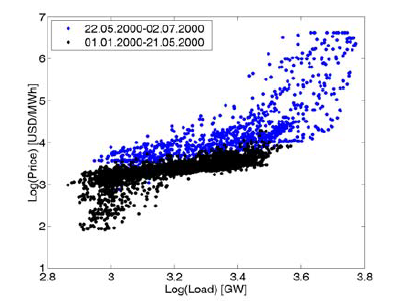
\includegraphics{figures/state_of_the_art/log_loads_vs_log_prices.PNG}
	\caption{The dependence between the
hourly log prices and hourly log system
loads in California for the period January 1
– July 2, 2000. \cite{weron2005forecasting}}
	\label{fig:log_loads_vs_log_prices}
\end{figure}

As can be observed the dependence between loads and energy prices is almost linear except for very low and very high loads, where electricity prices tend to jump to lower and higher values, respectively. 

Results show that for the proposed dataset ARX models (AR with exogenous variables) exhibit lower mean weekly errors (MWE) than AR models which in turn had significantly lower errors than standard ARIMA models. The difference is the separate modeling of individual hours for the ARX and AR models as opposed to an 48 hour aggregate modeling for ARIMA models. 

\subsection{ARIMA models to predict next-day electricity prices}

The authors in \cite{contreras2003arima} propose the application of ARIMA models for day ahead energy price forecasting based on data in the Spanish and Californian power markets. These models are based on time series analysis and results show that accurate electricity price forecasting for the aforementioned power markets is possible. Depending on the market and selected time range average weekly prediction errors 
range from 5\% to 10\%. These results are quite reasonable given that prices from the Californian market in the year 2000 have been selected which has been a very volatile and unstable time period due to the market crash in early 2001 \cite{weron2007modeling}. 

The described model generation process consists of five steps: 

\begin{itemize}
	\item[0)] A class of models is formulated assuming certain hypotheses.
	\item[1)] A model is identified for the observed data.
	\item[2)] The model parameters are estimated.
	\item[3)] If the hypotheses of the model are validated, go to Step 4, otherwise go to Step 1 to refine the model.
	\item[4)] The model is ready for forecasting.
\end{itemize}

This process is taken from the Box Jenkins methodology for forecast model generation \cite{hibon1997arma}.

Interestingly only five hour training periods are needed to model forecasts for the next consecutive hour for Spanish power prices, only two hour training periods are needed for modeling Californian energy prices. 
Through outlier detection the resulting forecasts could have been slightly improved but as stated in \cite{contreras2003arima} this would result in significantly increased computation time. 

%The first step (0) consists of determining a suitable class of models that can be applied to the time series based on observed characteristics, e.g.~high frequency, nonconstant mean and variance, and multiple seasonality. The hypothesis of the model at this step assumes a forecast error term with a normal distribution having a zero mean and constant variance. 
%
%In step 1) a trial model has to be selected for which data has to be made stationary. Through application of a logarithmic transformation a more stable variance can be achieved whereas (seasonal) differencing of data may result in a more stable mean. In order to find appropriate autoregressive and moving average coefficients for the resulting ARIMA model autocorrelation (ACF) and partial autocorrelation (PACF) plots may be consulted to retrieve a first fit of the model. 
%
%Step 2) consists of estimation of parameters which is typically done by applying the maximum likelihood function with respect to the parameters. In order to optimize forecasting performance outlier detection methods may be applied to minimize the impact of single "`spikes"' in the data. 
%
%In step 3) the residuals (forecast errors) of the resulting model are evaluated based on desired characteristics. Residuals should exhibit zero mean, constant variance, should follow a normal distribution and should be uncorrelated. Suitable tests for these properties are portmanteau tests (Ljung box, Box Pierce) and examination of ACF and PACF plots to find dependencies within the data. 
%
%Step 4) is concluding the model selection process. The resulting model of step 2) is used for forecasting based on trained data. 




\subsection{Energy price forecasting approaches in wholesale power markets}

According to \cite{lora2007electricity} electricity price models in general can be classified in two different sets of models, production cost models and statistical models. 

Production cost models retrieve all available information to accurately model system behavior while statistical models are trained on historical data and have little information about the underlying system. An advantage of statistical models is that the amount of information needed to build models is significantly less than that needed for production cost models. 

A taxonomy of electricity price forecasting models is presented in \cite{aggarwal2009electricity} (Figure \ref{fig:classification_of_price_forecasting_models}). 

\begin{figure}[htbp]
	\centering
		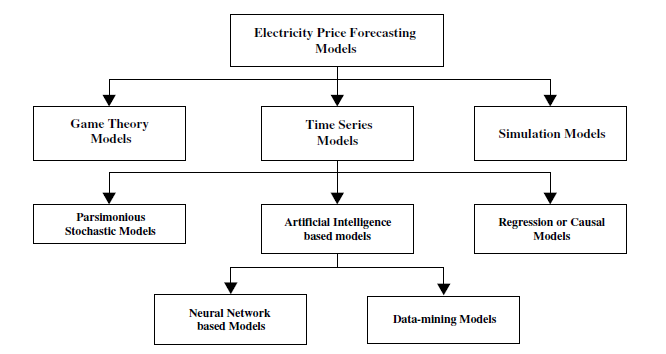
\includegraphics{figures/state_of_the_art/classification_of_price_forecasting_models.PNG}
	\caption{Classification of price forecasting models \cite{aggarwal2009electricity}}
	\label{fig:classification_of_price_forecasting_models}
\end{figure}

In the above taxonomy production cost models are all but parsimonious stochastic models and regression or casual models. Statistical time series models can thus be classified in classical time series models and models based on machine learning approaches \cite{lora2007electricity, duanelectricity}. Classical time series models have the benefit to exhibit a simpler structure than machine learning models, however it is hard to obtain accurate forecasts for non-linear time series such as energy prices. 

Regarding machine learning approaches, artificial neural networks (ANN) have been studied extensively in relation to electricity price forecasting \cite{vahidinasab2008day, singhal2011electricity, pao2007forecasting, amjady2006day, catalao2007short, 
gareta2006forecasting, duanelectricity, szkuta1999electricity}. Neural network models are trained to model non-linear relationships between applicable input variables and historical energy prices. 

Extensive research has been made regarding stochastic time series models as well whereby models may be applied to single \cite{garcia2005garch, weron2008forecastingWh, weron2008forecasting, nogales2002forecasting, cuaresma2004forecasting, tan2010day, conejo2005day} or complex multiple seasonality patterns \cite{de2011forecasting, gould2008forecasting, zivot2003vector}. 
Studies show that univariate time series models may be improved significantly by modeling each hour of the day separately \cite{cuaresma2004forecasting, weron2008forecasting}. However this requires model building separately for each hour which increases the amount of effort needed especially in dynamic forecasting environments. 
It is also stated that including modeling of non-linear phenomena would drastically increase computation time for time series models \cite{cuaresma2004forecasting}. 

%models may be classified in two types: univariate and multivariate time series models. 

Results show that ANN models have the potential to outperform statistical models such as Autoregressive (AR) or Autoregressive Integrated Moving Average (ARIMA) models \cite{pao2007forecasting, catalao2007short}. This may be due to their ability to more accurately model the underlying system behavior while they excel at modeling non-linear relationships in the dataset. 

However, in order to successfully apply forecasting based on neural network models a set of requirements have to be met \cite{catalao2007short}: Availability of sufficient amounts of data, adequate selection of input/output samples, an appropriate number of hidden units and sufficient computational resources. In case these requirements can not be met or it is not possible to appropriately parametrize the model statistical models provide a good alternative for modeling energy prices. 




\section{Cost optimization in geo distributed data centers}

%Different cost optimization approaches have been developed for distributing resources in geographically dispersed data centers. 

\subsection{A Study of Electricity Price Features on Distributed Internet Data Centers}

A comprehensive study about optimization of energy costs under different operational and energy cost prediction regimes is presented in \cite{de2013study}. 

The focus of this work is to leverage price differences across different energy markets in a network of geo distributed data centers to minimize energy costs by migrating resources to currently cheaper locations. It takes into account the impact of several metrics including the level of price variability, time lag between locations, reconfiguration delay and accuracy of energy price predictions. 

To provide a forecasting model based on the given data the Box-Jenkins method is used to build an ARIMA model characterizing the underlying electricity price data:

\[ ARMA(p,q) : P_t = \epsilon_t + \sum_{i=1}^{p}{\phi_i P_{t-i}} + \sum_{j=1}^{q}{\theta_j \epsilon_{t-j}}\] 

where $p$ and $q$ are the number of autoregressive and moving average terms, $\phi_i$ and $\theta_j$ denote the model coefficients and $\epsilon_t$ denotes the error term at time $t$. To accurately model seasonality in the data an $SARIMA(p,d,q)(P,D,Q)[s]$ model has been used which includes the number of terms $p,q$ and $P,Q$ as non-seasonal and seasonal parameters and $d$ and $D$ for non-seasonal and seasonal differencing, respectively. 

Price time series have been generated with different levels of variability $\sigma_{Price}^{2} \in \{50, 126.6, \ab 300, 500\}$. In addition, prediction errors have been used to simulate different forecast accuracy levels, $\sigma_{pred} \in \{2.0, 5.0, 10.0\}$. 

Thus, $P = \{p_1,\ldots,p_T \}$ denotes a price time series and $\hat{P} = \{\hat{p_1},\ldots,\hat{p_T}\}$ a simulation of forecast values such that 
$\hat{P_t} = \mathcal{N}(P_t, \sigma_{pred}), \forall t \in T$. As a measure of accuracy the mean squared error (MSE) has been used: 
$MSE(P,\hat{P}) = \frac{1}{T} \sum_{t \in T}{(P_t - \hat{P_t})^2}$. 

The decision of workload assignment at a particular time $t$ is based on the number of active servers at location $i$ and the corresponding forecast prices $\hat{P_i}(t)$. The total cost at any given moment is defined by $\hat{C_t} = \sum_{i=1}^{N}{m_i \times \hat{P_i}(t) \times Po_i}$ where $Po_i$ denotes the power used by a server running at location $i$ and $m_i$ defines the number of running servers at location $i$. 

Results for different metrics achieved different cost savings \cite{de2013study}. When the number of locations involved in the simulation is increased, cost savings up to 10\% have been reported when going from 1 up to 20 locations. The more locations are considered the greater benefit can be drawn from price differences and time lags between different locations. 

Price variability has been simulated with $\sigma_{price}^{2} \in \{0,5,\ldots,500\}$ and resulting costs have been estimated. It was shown that up to 15\% of savings could be achieved when comparing the maximum and minimum simulated price variabilities. 

Concerning time lags it is stated that the most benefit could be drawn from locations in timezones that are sufficiently distant from each other due to the daily seasonality observed in energy prices. For this scenario up to 15\% cost savings have been achieved for locations that were perfectly "`out of phase"'. 

Finally results show that forecast errors have a major impact on resulting costs. In order to quantitatively measure the impact of forecast deviations $\sigma_{pred}$ has been increased stepwise in the range $0,\ldots,5$ by steps of $0.1$.
The resulting MSE is quadratically rising with the level of $\sigma_{pred}$, thus when errors are at maximum a 10\% revenue loss is expected. 
Therefore accurate forecasts are very important to achieve major cost savings in a multi cloud environment. 




\subsection{Cutting Down the Energy Cost of Geographically Distributed Cloud Data Centers}

This paper aims to minimize energy costs in geographically distributed data centers by taking into account spatio-temporal variation in electricity prices and the outside weather temperature \cite{guler2013cutting}. The scenario is modeled as a linear programming problem which is solved by presenting various heuristic solutions to the problem. 

While providing algorithms for minizing energy costs resulting SLA penalties as well as cooling related costs are taken into account. 
For each data center a performance coefficient (CoP) is calculated which is based on outside weather temperature where the coefficient increases linearly with rising temperature. A data center may have different types of servers exhibiting different performance metrics and capacities. 

Energy costs are calculated as the sum of server power consumption over a specific time range multiplied by the applicable energy prices during that time. 
The total costs for data center $i$ are defined as $E_{i}^{total} = E_{i}^{IT} \times CoP(T_i)$ where $T_i$ denotes the temperature at location $i$. 

The actual time a job $j$ needs when running on a type $k$ server $s$ is defined as 
\[  T_{j,s} = \frac{c_j \times f_j \times l_j}{c_k \times f_k}  \] 
where $c$ and $f$ denote the number of cores and frequency available / needed by a server / job and $l$ denotes the expected runtime of job $j$. 
A penalty occurs if the total runtime of a job exceeds the expected runtime when running on server $s$. 

The goal is to minimize the sum of total energy and penalty costs over all data centers 
\[ \min \sum_{i=1}^{N}{E_{i}^{total} + Pen_i} \]
where $Pen_i$ denotes the total penalty cost for data center $i$. 

Based on the proposed linear optimization problem two types of scheduling algorithms are introduced, immediate and delayed. Immediate scheduling algorithms are defined as CheapestDC and CheapestS where the former places resources randomly on hosts located at the currently cheapest data center while the latter includes outside weather temperature as well in the calculation. Delayed scheduling algorithms additionally consider historical energy prices to decide whether jobs should be delayed to a future time stamp. 

Simulation runs over six data centers at different locations handling three types of workloads were conducted to evaluate different scheduling algorithms.
Results show that delayed scheduling techniques on light workloads achieve over 5\% on overall cost savings compared to the baseline random scheduler. Also, spatial electricity price variations have the most impact on cost savings followed by temporal electricity price changes and reduced cooling costs due to outside weather temperature. 


\subsection{Studies for cost optimizations in multi-electricity-market environments}

Different studies have been developed for optimizing energy costs in multi market environments. 

In \cite{buchbinder2011online} the basic tradeoff between energy and bandwidth costs is discussed for migrating virtual machines between geographically distributed data centers. 
Three different algorithms have been evaluated on a set of 30 US locations covering three years of next day electricity data. Out of the two greedy algorithms and the online migration algorithm the latter provided the best results with only 4 to 6 \% off the optimal offline solution. 

The authors in \cite{rao2010minimizing} aim to minimize energy costs while guaranteeing quality of service by referring to a constrained mixed integer programming model. The approximated linear programming model is converted to a minimum cost flow problem which can be solved fast and efficiently. With five frontend web portal servers targeting three internet data centers cost reductions up to 30\% are achieved within the simulation. 

An extensive study on electricity price features and its implications for existing cloud systems is given in \cite{qureshi2009cutting}. While taking into account server energy elasticity and bandwidth constraints a maximum cost savings of 45\% could be achieved when running a simulation over 39 months including 29 locations. However, in order to achieve these results bandwidth constraints are relaxed and large distances to clients have to be permitted. 

A different approach is examined by \cite{simarro2011dynamic} where dynamic pricing schemes of different cloud providers are taken advantage of to reduce investment of users. The assumption is that prices for each cloud provider change according to demand and thus virtual cluster placements can be optimized across different cloud providers. As infrastructure is dynamically distributed without notice of the user it provides an efficient and convenient way of reducing costs for cloud users. 

Cost based multi cloud schedulers have been investigated in \cite{le2009cost} and \cite{tordsson2012cloud}. 
A cloud scheduler for simplified management of virtual machines has been developed in \cite{armstrong2010cloud}, a green cloud scheduler in \cite{lucanin2013take}. 
Also, schedulers based on genetic algorithms were proposed by \cite{dutta2011genetic} for cost based multi QoS optimizations and \cite{ge2010ga} for improving delay scheduling policy. 



\section{Optimize resource scheduling in data centers}

\subsection{A task scheduling algorithm based on load balancing in cloud computing}

In \cite{fang2010task} a two level scheduling model has been implemented (Figure \ref{fig:two_level_resource_scheduling}). 

\begin{figure}[htbp]
	\centering
		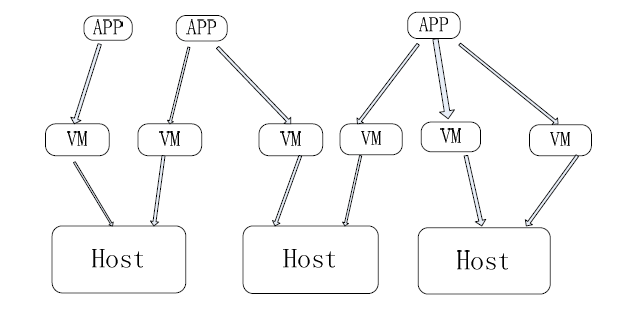
\includegraphics[width=0.7\textwidth]{figures/state_of_the_art/two_level_resource_scheduling.PNG}
	\caption{Two level scheduling model \cite{fang2010task}}
	\label{fig:two_level_resource_scheduling}
\end{figure}

A two stage process is described where the first scheduler creates the task description of a virtual machine s.t.~the task will have a perfect fit on a virtual machine whereas the second scheduler is responsible to find appropriate resources (hosts) for the provisioned virtual machine. Thus an optimized resource scheduling is presented with focus on load balancing among different clouds. 

Tasks have a defined structure where task $t_i$ out of the set of all Tasks $T$ is defined as 

\[t_i = \{tId, tRr, tSta, tData, tVmch, tVm\}\]

\begin{itemize}
	\item $tId$ is the task identification
	\item $tRr$ denotes the required resources
	\item $tSta$ describes the state of the task where $tSta = \{tFree,tAllo,tSche,tWait,tExec,tComp\}$
	\item $tData$ defines the relative data of the task (computational load, input and output data)
	\item $tVmch$ denotes the virtual machine specification where $tVmch = \{tId,tRr,tData\}$
	\item $tVm$ defines the assigned virtual machine of the task where $tVm = \{tId,thId\}$
\end{itemize}

Hosts on the other hand are defined as $h_j = \{hId, hTcap, hFcap, hData\}$, where

\begin{itemize}
	\item $hId$ denotes the host identification
	\item $hTcap$ is the total host capacity (set of resource capacities)
	\item $hFcap$ is the freely available host capacity
	\item $hData$ denotes the relative data of the host (including input and output bandwidth)
\end{itemize}

%Concerning the scheduling algorithm, the predicted task resource usage is defined as $VL_i$. 

The scheduling algorithm is based on the following equations: 

\[ HL_i = \frac{\sum_{j=1}^{n}{VL_j}}{n} \]

\[ avgl = \frac{\sum_{i=1}^{m}{HL_i}}{m} \]

\[ B = \frac{\sqrt{\sum_{i=1}^{m}{(HL_i - avgl)^2}}}{m} \]

where $VL_j$ is the predicted resource load for VM $j$, $HL_i$ is the average load for host $i$, $avgl$ denotes the average
load across all running hosts and $B$ denotes a metric for load balancing. 

The scheduler iterates over the set of hosts in each timestamp and determines the value of the load balancing metric $B$. In case the value of 
$B$ exceeds a predefined threshold $B_0$ or the predicted resource requirements for a virtual machine exceed the currently allocated resources 
the VM is migrated to a host occupying the least resources for optimal load balancing. 

Results show that considering dynamic resource requirements load is distributed across all machines leading to stable level of cloud utilization. 



\subsection{Efficient resource management for cloud computing environments}

In \cite{younge2010efficient} power aware and live migration scheduling techniques are proposed as a green cloud approach to increase overall system efficiency with minimal performance overhead. 

A new greedy based algorithm is presented to minimize power consumption. It is based on the findings that power consumption of a server does not increase linearly with the number of cores utilized. Instead, most power is drawn by one utilized core whereas power increases only slightly when comparing a server utilizing 7 to 8 cores. Thus a new VM scheduling algorithm is proposed that minimizes resulting power consumption within a data center. 

Hosts are assigned to a pool of resources where a pool can be initialized by a priority based evaluations system to either maximize performance or further minimize power consumption \cite{younge2010efficient}. Each VM request is checked against its resource requirements and available capacities in the pool and assigned to a host to maximize utilization and therefore minimize overall power consumption. 

In addition, live migration of virtual machines is applied to further optimize power consumption by shifting load away from under utilized hosts (Figure \ref{fig:server_power_consumption}). When load increases, Wake on Lan (WOL) technology is used to power servers back up again. Furthermore, a focus has been to reduce VM image size and boot time to optimize virtual machines for a server environment. 

%\begin{figure}[htbp]
	%\centering
		%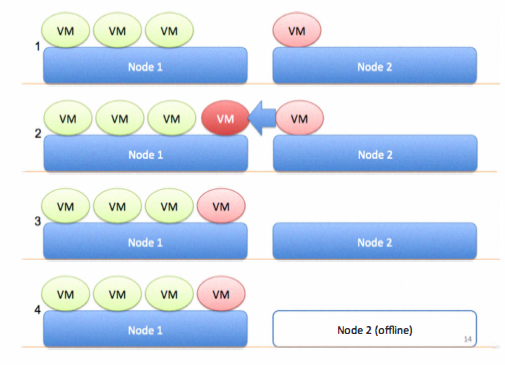
\includegraphics{figures/state_of_the_art/vm_migration_for_host_consolidation.PNG}
	%\caption{Virtual machine management dynamic shutdown technique \cite{younge2010efficient}}
	%\label{fig:vm_migration_for_host_consolidation}
%\end{figure}

\begin{figure}[htbp]
	\centering
		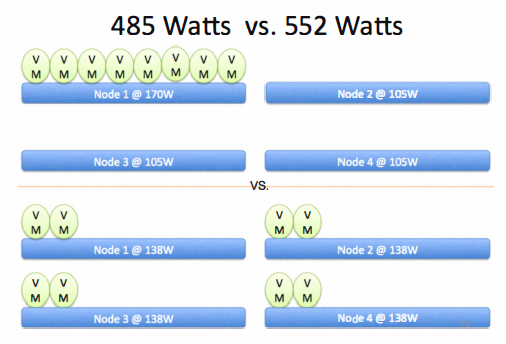
\includegraphics{figures/state_of_the_art/server_power_consumption.PNG}
	\caption{Illustration of scheduling power savings \cite{younge2010efficient}}
	\label{fig:server_power_consumption}
\end{figure}

Power aware resource scheduling has been simulated on an OpenNebula \cite{fontan2008opennebula} pool of 4 servers, equipped with 8 cores each. Power elasticity (power range from idle to peak power of a server) for this type of server is 61\% where a total reduction in power consumption of 12\% could be achieved. As the results are scalable also to large clusters significant power and cost savings are possible using the proposed approach. 


%
%Active research topics in this field include electricity cost reduction in data centers \cite{guler2013cutting, le2011reducing}. A comparison of different approaches considering spatial and temporal energy price changes and the contribution of the outside temperature to the resulting cooling effort and expense is outlined in \cite{guler2013cutting}. In \cite{le2011reducing} a set of homogenous data centers is simulated where the focus lies on the effects of changing workloads and migrations on the cooling infrastructure and on intelligent scheduling to reduce energy consumption and energy costs, respectively. 
%
%The authors in \cite{lucanin2013take} propose a green cloud approach using real time electricity prices where the duration and time of price peaks are estimated and VMs are paused during these times to reduce energy costs and save energy. Customers may choose between ``green'' and normal instances, taking into account some loss of availability for a reduced price. 
%
%
%
%In \cite{rao2010minimizing} a cloud consisting of several Internet Data Centers (IDC) is examined with regard to cost optimization which is done by intelligently assigning workload to data centers based on current energy prices. Two of these data centers in the scenario are connected to deregulated wholesale energy markets whereas the other one is connected to a regulated utility region charged by a fixed pricing scheme. Since price change differences in deregulated energy markets can be considerable energy cost reductions may be achieved by assigning workload based on changing energy prices.  %For the purpose of the simulation five front-end Web portal servers process a total workload of about $10^5$ requests per second. 
%
%In this paper the approaches of optimal and average workload assignments are visually and formally compared to gain insights into the total electricity cost reduction. The optimal workload assignment is calculated with respect to workload and delay constraints that are considered in a minimum cost flow problem based on a linear programming model. Thus the goal is to minimize costs without compromising quality of service constraints. 
%%The proposed cost reductions amount up to 30 percent for a single hour test within the given time range. 
%%The results measured at two timestamps at a specific day seem promising, since total cost reductions could be achieved by 30\% and 17\% respectively. 
%
%The differences compared to this work is that in \cite{rao2010minimizing} they do not consider longer running jobs as used in scientific calculations or large optimization problems that may take several hours to complete. Thus the impact of migrations is not examined in this scenario. In addition the possibility of energy price forecasting is not considered which may result in even greater energy cost reductions. 
%
%Another study on cost reductions in Internet Data Centers has been done where different aspects of cost reductions including cost prediction schemes have been considered \cite{de2013study}. Since up to 15\% of total capital investment is spend on energy related costs 
%%(paper references \cite{greenberg2008cost} - old, from 2009!!) 
%a special effort is invested to reduce the amount of energy costs through cost aware operations. %(TODO: Move to introduction?)
%
%In this paper cost optimization is seen as an assignment problem where an overall cost function is minimized through intelligent workload allocation. During the investigation different variables and their impact on resulting energy costs are considered which are price volatility, price predictions including variable prediction errors, time lag between locations and reconfiguration delays. 
%
%Similar to this work the simulation is run with the same set of fixed parameters to evaluate the impact of the various scenarios. It is observed that prediction errors greatly impact workload allocation where cost penalties due to non-optimal assignments increase quadratically with an increase of forecast errors \cite{de2013study}. Also with increasing number of locations the minimum cost of optimal assignments can be greatly reduced. Greater price volatility is beneficial as well since then price aware assignments will have greater impacts. 
%
%A comprehensive study on cost reductions and energy market characteristics in an environment where data centers are placed within the reach of different energy markets is presented at \cite{qureshi2009cutting}. Based on geotemporal variations of energy prices the maximum cost reductions under different scenarios are evaluated. Energy expenses are estimated for various large scale companies like Google and Yahoo to state the actual savings and the amount of reductions in energy costs that would be possible. 
%They also discuss the impact of considering bandwith constraints and maximum client server distances on cost reductions. 
%
%Interestingly enough long term seasonalities in the energy price data has been discovered that spanned multiple energy markets. This is an important fact when training forecasting models since predictions can become a lot more accurate. An important fact that was revealed about energy markets was that data from different energy markets was much less correlated than data from the same area. Thus to take full advantage of energy price differences data centers located at different energy markets should be combined \cite{qureshi2009cutting}. 
%
%With different state of the art energy models and simulation constraints a summary of possible cost reduction schemes was presented. However no migration or forecasting of energy price data has been done which could further improve scenarios with longer running jobs. In addition these cost reductions are only valid under specific assumptions that large cloud providers would need to implement such as connection to wholesale energy markets and reasonable server energy elasticity. 
%
%
%
%
%\subsection{Server power management}
%
%A well known problem in power management is how to accurately and efficiently model a server's power consumption over time. At \cite{horvath2008multi} Horvath et al.~exploit dynamic voltage scaling (DVS) and multiple sleep states to reduce power consumption of a server cluster of about 23\% without significantly impacting performance. They propose that CPU utilization and frequency are the variables that have the most significant impact on the power consumption of a machine. This assumption is also used in other studies, e.g.~\cite{rao2010minimizing, hammadi2014survey, kliazovich2012greencloud}. 


\section{Virtual machine migration}
%\subsection{Virtual machine migration in cloud environments}


Live Virtual machine migration is defined as follows:
\begin{quote}
A source virtual machine (VM) hosted on a source server is
migrated to a destination VM on a destination server without
first powering down the source VM \cite{nelson2009virtual}.
\end{quote}

Thus efficient methods for transferring VM memory pages from the source to the destination host are needed which will be evaluated in the following sections. 
%One method is defined by resuming the destination VM before all memory pages from the source VM are transferred. This can be done by paging in any remaining VM memory pages from the source to the destination on demand. A second approach executes a pre-copy phase where memory is transferred in several rounds from the source to the destination host before launching the destination VM. Dirtied memory pages are re-transferred which have been dirtied during previous transfers of memory to ensure a consistent VM memory image at the destination. 
%
%The non-memory state of the VM is preferably available in a shared storage arrangement accessible by both the source and destination VMs such that it is only required to re-map the source VM's virtual disk to the destination VM. In case no shared storage is available, the source VM's non-memory state has to be transferred to the destination VM before or after the migration depending on the implementation. 


\subsection{Live migration of virtual machines}

In \cite{clark2005live} an efficient approach for live migration of virtual machines is presented. This paper targets the migration of entire OS within a virtual machine without noticeable service interruption. 

The applied method for migration should minimize both downtime and total migration time for the virtual machine. The first metric denotes the actual downtime of the VM where it is completely suspended and unaccessible to users. The second metric is defined by the total time between the start of the migration process until its end \cite{clark2005live}. 

Three methods have been identified that have been used previously. The \textit{pure stop-and-copy} approach halts the source VM, copies all memory pages to the destination host and resumes execution at the destination. Both downtime and total migration time are proportional to the amount of memory to be transferred which can lead to unacceptable downtimes. 

The \textit{pure demand migration} method is defined where essential data for running the VM is transferred to the destination host after which the destination VM is booted. Any missing memory pages create page faults and trigger a synchronous transfer from the source host on first use. This leads to poor performance until a sufficient amount of memory pages have been transferred. 

The \textit{pre-copy} approach combines an iterative push-phase with a very short stop-and-copy phase to minimize downtime. Any pages dirtied during a transfer of memory are re-sent in the next iteration until a sufficient amount of memory pages have been transferred to the destination host. In a final stop-and-copy phase the VM is suspended on the source host, remaining memory pages are copied to the destination and the VM is resumed at the destination. 

An important efficiency measure for VM migrations has been identified as the writable working set (WWS) \cite{clark2005live}. It is defined as a set of memory pages that are updated very frequently such that it is not worth keeping them consistent at the source and destination hosts. These set of pages should be copied only in the final stop-and-copy phase. An accurate measure of the WWS for the SPEC CINT2000 benchmark is depicted in Figure \ref{fig:tracking_writable_working_set}. 

In this graph the number of 4KB pages of memory dirtied within a corresponding 8 second interval are shown for each of the programs run in the benchmark. 
It is clearly visible that the number of pages contained within a WWS depends greatly on the behavior of the selected program. Workloads exhibiting a high amount of frequently updated pages such as \textit{gap} will provide only a small number of pages sensible for inclusion in a pre-copying phase. 
Thus the downtime and cost resulting from a VM migration depends to a great extent on the type of workload being migrated and the exact moment of the start of the migration. 

%Thus the source virtual machine does not hold any dependencies related to the destination VM after migration has finished. The in-memory state of the VM is transferred efficiently such that a seamless live migration becomes possible. 


\begin{figure}
	\centering
		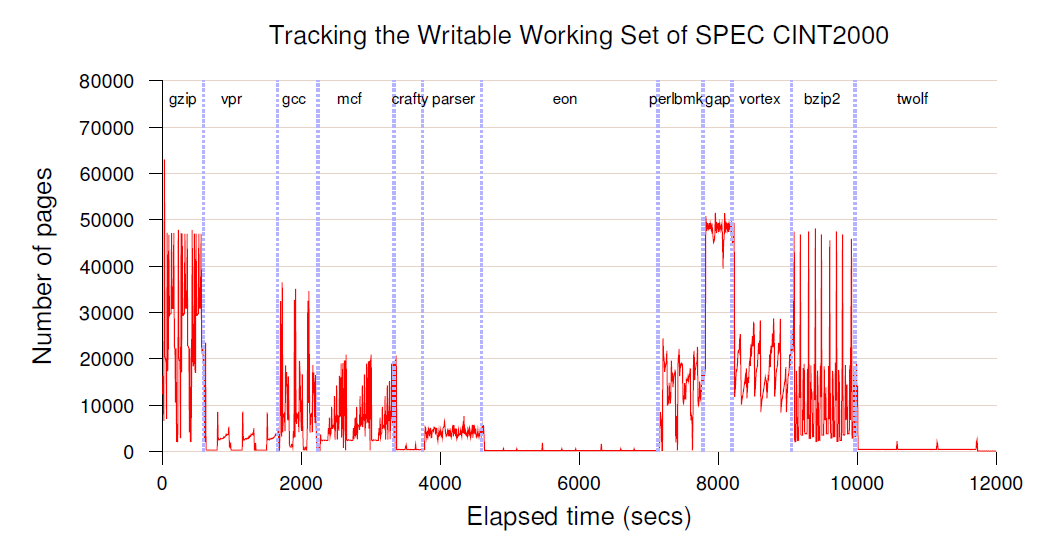
\includegraphics[width=1.0\textwidth]{figures/state_of_the_art/tracking_writable_working_set.PNG}
	\caption{WWS curve for a complete run of SPEC CINT2000 (512MB VM) \cite{clark2005live}}
	\label{fig:tracking_writable_working_set}
\end{figure}



Results for different kind of workloads indicate that even in the worst case the pre-copy approach significantly reduces downtime compared to the stop-and-copy method. As bandwidth has a direct impact on migration downtime performance can be further increased by raising the bandwidth assigned to the VM migration. 

Migration downtimes have been evaluated for different sized VMs running various kinds of workloads. Resulting downtimes range from only 60 ms for small sized VMs (64 MB) and low dirty page rate to 3.5 seconds for large VMs (512 MB) with frequently updated dirty page rates. It is stated that realistic workloads can be migrated with a downtime as low as 210 ms in a virtualized cluster environment. 


\subsection{Performance and energy modeling for live Migration of Virtual Machines}

A thorough evaluation of migration performance and resulting migration costs is given by \cite{liu2013performance}. 

The authors provide methods to quantitatively predict migration performance and resulting energy cost. A refined pre-copy approach is used to efficiently transfer memory pages in iterative rounds where in each round the memory pages dirtied in the previous round are re-sent (Figure \ref{fig:VM_migration_precopy}). 
The pre-copying phase is terminated when any of the following conditions are satisfied:

\begin{enumerate}
	\item [1)] memory dirtying rate exceeds memory transmission rate
	\item [2)] the remaining dirty memory falls below a predefined threshold
	\item [3)] the number of pre-copying iterations exceeds a defined maximum
	\item [4)] total network traffic exceeds a multiple of the VM memory size
\end{enumerate}

\begin{figure}[htbp]
	\centering
		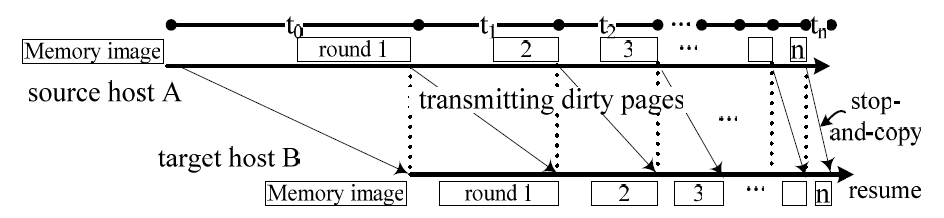
\includegraphics[width=0.7\textwidth]{figures/state_of_the_art/VM_migration_precopy.PNG}
	\caption{Live migration algorithm performs pre-copying in iterative rounds \cite{liu2013performance}}
	\label{fig:VM_migration_precopy}
\end{figure}

Findings in this work include that with incremental data transmission rate (bandwidth) the power consumption progressively increases while the migration latency decreases. Also, power consumption during migrations increase for both source and destination hosts from which the resulting migration energy can be derived. In addition the migration load and time needed for each pre-copy iteration as well as the total migration load and latency are calculated. 

Besides the defined base model a refined migration model is specified which takes into account the size of a workload's writable working set, that is the number of pages dirtied most frequently. The latter model has been empirically evaluated by measuring the WWS on a Xen virtual machine and deriving the maximum sensible pre-copy iteration while continuously checking termination conditions. 

\begin{figure}[htbp]
	\centering
		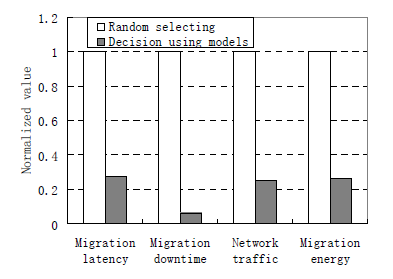
\includegraphics{figures/state_of_the_art/vm_migration_normalized_cost.PNG}
	\caption{Migration cost savings by using proposed models \cite{liu2013performance}}
	\label{fig:vm_migration_normalized_cost}
\end{figure}

Workloads with different sizes for writable working sets have been evaluated in simulations including two hosts running 8 virtual machines. 
The resulting migration downtime, migration latency, network traffic and energy consumption could be reduced by 72.9\%, 93.5\%, 74.5\% and 73.6\% compared to a random selection technique, respectively (Figure \ref{fig:vm_migration_normalized_cost}). 





%Migration costs and downtime may vary significantly depending on the type of workload and VM configuration parameters. The authors leverage cost prediction schemes to yield expected costs for specific VM migrations. 









%See "`Live Virtual Machine Migration via Asynchronous Replication and State Synchronization"'
%
%\begin{figure}[htbp]
	%\centering
		%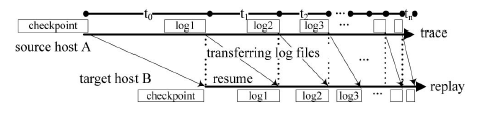
\includegraphics{figures/state_of_the_art/virtual_machine_precopy.PNG}
	%\caption{Migration process ideal case}
	%\label{fig:virtual_machine_precopy}
%\end{figure}

%
%\begin{figure}[htbp]
	%\centering
		%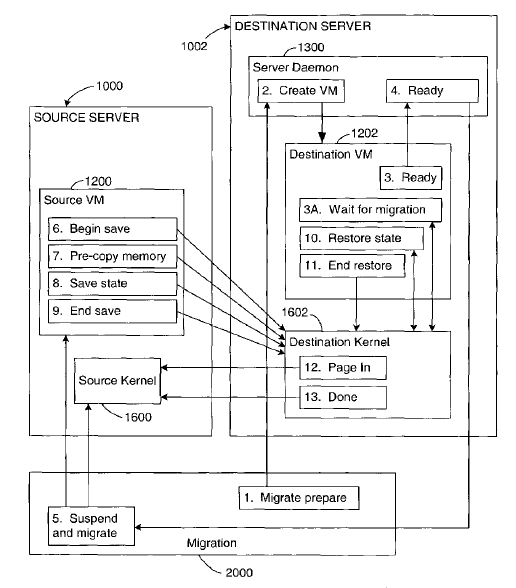
\includegraphics{figures/state_of_the_art/virtual_machine_migration.PNG}
	%\caption{Virtual machine migration}
	%\label{fig:virtual_machine_migration}
%\end{figure}


%There are different proposed approaches related to virtual machine migration in distributed cloud environments \cite{celesti2010improving, malet2010resource}. In \cite{celesti2010improving} the so-called Composed Image Cloning (CIC) methodology designed for migration of VMs across federated clouds is introduced. This work aims to reduce the needed bandwidth and migration time by setting up a new virtual machine in the destination cloud and transferring only user data instead of relocating the whole VM disc image. 
%
%In another work \cite{malet2010resource} the placement of applications is dynamically adjusted across distributed data centers according to the location of the currently highest request rate. 




%%%%%%%%%%%%%%%%%%%%%%%%%%%%%%%%%%%%%%%%%
\chapter{Data Analysis}
\label{ch:data_analysis}
%%%%%%%%%%%%%%%%%%%%%%%%%%%%%%%%%%%%%%%%%





\section{Day ahead and real time energy prices}




\section{Characteristics of energy markets}

Ideas: 

\begin{itemize}
	\item Show electricity price variation for market over a 3 year period (Weron, pg 33)
	\item Show autocorrelation function over extended (same) time period
	\item Show periodogram over extended time period
\end{itemize}




See folders "`Electricity pricing"' and "`power markets"'


\begin{figure}[htbp]
	\centering
		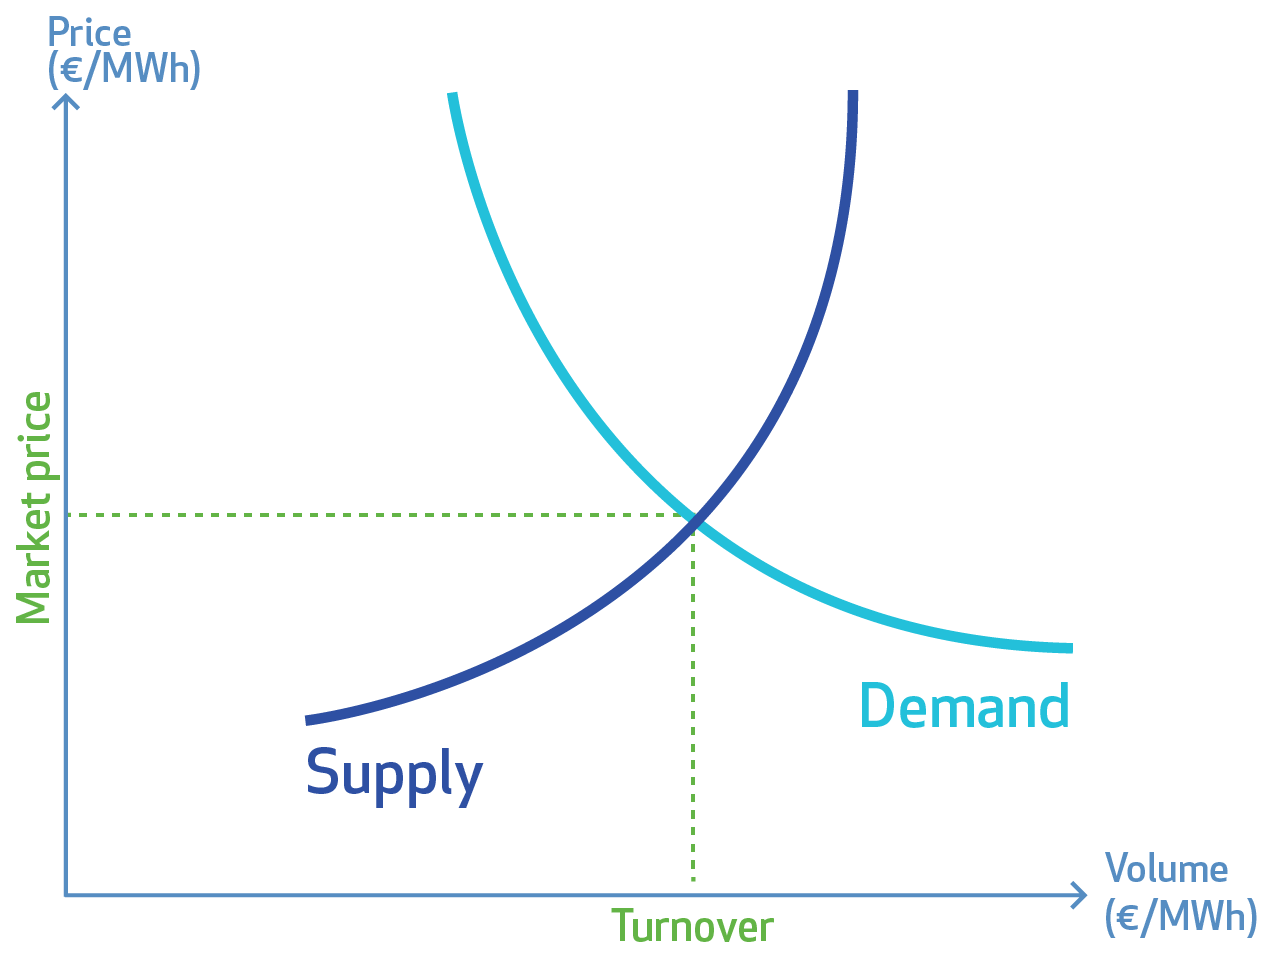
\includegraphics[width=0.5\textwidth]{figures/data_analysis/DA_supply_demand.png}
	\caption{Intersection between supply and demand \cite{nord2014supply}}
	\label{fig:DA_supply_demand}
\end{figure}



In this section different studies of power market characteristics are presented to distinguish features that may be used in building forecasting models. 

\subsection{Stable Modeling of different European Power Markets}

In this paper different European power markets have been investigated to reveal major differences in energy price behaviour \cite{mugele2005stable}. The EEX, Nord Pool Spot and Polish power markets have been evaluated whereby the markets are responsible for the Mid-Europe, Northern Europe and Polish regions respectively. 

As in general electricity prices depend on energy demand \cite{weron2005forecasting} which changes due to climate conditions (temperature and number of daylight hours) electricity prices exhibit a seasonal component as well (Figure \ref{fig:seasonal_behaviour_of_eex_prices}). 

\begin{figure}[htbp]
	\centering
		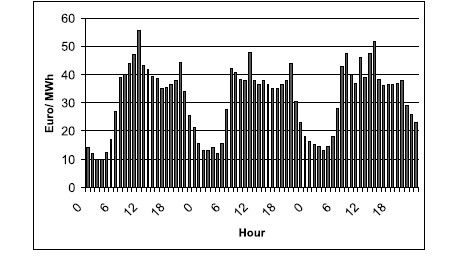
\includegraphics{figures/state_of_the_art/seasonal_behaviour_of_eex_prices.PNG}
	\caption{EEX - hourly spot prices \cite{mugele2005stable}}
	\label{fig:seasonal_behaviour_of_eex_prices}
\end{figure}

The main differences between electricity power markets and other financial markets are price volatility, mean reversion and price jumps or "`spikes"'. Volatility is high as generated electricity cannot be stored but has to be delivered at once which might lead to high prices on transmission congestion or surges in demand. It's impact can be reduced by applying logarithmic transformations of input data \cite{weron2005forecasting}. 

Energy prices experience strong mean reversion which denotes the characteristic that prices return to their mean levels after an increase in prices. In addition price spikes may appear where prices can increase tenfold from one hour to the next. To mitigate these spikes they may be averaged out in a data preprocessing step. 

Even though price seasonality and trend seem to be stable over a short time range (Figure \ref{fig:seasonal_behaviour_of_eex_prices}) they can show significant fluctuations over a longer time range. In \cite{mugele2005stable} data related to each examined energy market was fitted to a stable Paretian distribution as well as a normal distribution. The result showed that mature markets as EEX or Nord Pool Spot exhibit high volatility, heavy tails, high kurtosis and asymmetrics in the energy price data which was best modeled by the Paretian distribution. In contrast the Gielda Energii SA market in Poland shows a much more stable energy price behavior which can be modeled by a Gaussian distribution. 

The variation in energy price levels for the two power markets EEX and Nord Pool Spot are shown in Figures \ref{fig:EEX_levels} and \ref{fig:NordPool_levels}.

\begin{figure}[!htbp]
  \centering
  \begin{minipage}[b]{0.4\textwidth}
    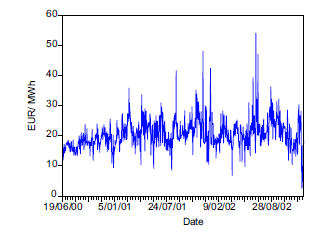
\includegraphics[width=\textwidth]{figures/state_of_the_art/EEX_levels.PNG}
    \caption{EEX levels \cite{mugele2005stable}}
		\label{fig:EEX_levels}
  \end{minipage}
  \hfill
  \begin{minipage}[b]{0.4\textwidth}
    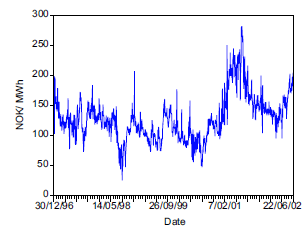
\includegraphics[width=\textwidth]{figures/state_of_the_art/NordPool_levels.PNG}
    \caption{Nord Pool levels \cite{mugele2005stable}}
		\label{fig:NordPool_levels}
  \end{minipage}
\end{figure}

This shows that it is important to investigate energy price characteristics from power markets to accurately model market prices. 



%
%\subsection{Electricity markets and pricing}
%
%In wholesale energy markets different pricing and bidding models can be used. Currently the two most common price evaluation strategies are day-ahead and real-time pricing strategies. 
%
%\subsubsection{Bidding strategies}
%
%In \cite{tierney2008uniform} two different bidding strategies are discussed, uniform pricing and pay-as-bid auctions. In the uniform pricing model the market clearing price is determined by collecting the marginal prices from all suppliers and taking the maximum price from this collection. Conversely, in pay-as-bid auctions a supplier gets paid based on its actual bid. 
%The second approach may seem beneficial from the customer's point of view since suppliers may set individual prices which enables competition within the market. 
%However studies show that in this pricing scheme suppliers set their prices at the maximum possible level to be comparable to other suppliers and keep their customers. On the other hand the uniform pricing model provides a uniform clearing price which is valid for all participants in the market and customers may trust that suppliers set prices to just satisfy their needs. 


\section{Energy price case study}





%%%%%%%%%%%%%%%%%%%%%%%%%%%%%%%%%%%%%%%%%
\chapter{Forecasting}
\label{ch:forecasting}
%%%%%%%%%%%%%%%%%%%%%%%%%%%%%%%%%%%%%%%%%


\section{Introduction}

As outlined in \ref{sec:electricity_price_forecasting} different types of models have been investigated for forecasting spot electricity prices. In this work forecasting models should be used that exhibit the following characteristics: 

\begin{itemize}
	\item computationally lightweight
	\item capable of modeling seasonality
	\item capable of recognizing trends in the dataset
	\item good out-of-sample accuracy based on day ahead and real time electricity prices
	\item capable of being part of an automated model generation process
	\item accurate modeling of different energy price characteristics
\end{itemize}

Statistical models have been proven to provide good results and at the same time keeping the computational effort low \cite{aggarwal2009electricity,bunn2003forecasting}. In contrast structural or non-parametric models require additional input data and perform more complex operations such that they might not be the optimal choice for dynamic forecast environments. Therefore models in this work have been chosen from the well known set of parsimonious stochastic models. 

Different stochastic models are able to generate forecasts while considering existing seasonality in the data \cite{gould2008forecasting,de2011forecasting}. Examples of models exhibiting these characteristics are SARIMA, HoltWinters and TBATS, all of which are investigated in this work to evaluate their capability of forecasting on different settings and datasets. The best model is then chosen to provide forecasts for all simulations described later in this work. 

In general time series may be decomposed into seasonal, trend and cycle components which can be made use of by forecast models \cite{de2011forecasting}. Some models such as ARIMA and TBATS can handle existing trends in the dataset by applying transformations in a preprocessing step or by decomposing and separately modeling time series components. More simplistic models such as Simple Exponential Smoothing (SES) or pure Autoregressive (AR) models require the dataset to be stationary, i.e.~to exhibit a constant mean and variance \cite{weron2007modeling,hyndman2012forecasting}. In this case the dataset would have to be transformed before applying those models. 

Models should provide good out-of-sample accuracy which means that they need to be trained and tested on different datasets \cite{hyndman2012forecasting}. For example, considering training data from a training period of four weeks of energy price data and test data from a subsequent test period of one week a model is trained based on that training data but tested on the provided test data. Thus real life forecasting scenarios can be established and models are evaluated based on the accuracy on test datasets. A large scale evaluation of forecasting models based on different trainings and test datasets is presented later in this section. 

Building an automated model generation process is important for automatic model evaluation and model selection for simulations running over a longer period of time. As extensive simulations including forecasts represent a core contribution of this work an automated model generation process has been defined including preprocessing steps and model evaluation to find the best suited model for a given dataset. 

Inclusion of energy price characteristics such as mean reversion and price spikes into forecast model generation has been studied extensively considering different types of forecast models \cite{weron2008forecasting,bunn2003forecasting,aggarwal2009electricity}. Mean reversion denotes the characteristic that a time series returns to its mean after significant deviation. This characteristic is modeled by a AR(1) process and can be incorporated e.g.~into an ARIMA model. For handling price spikes three approaches have been defined in literature \cite{weron2008forecasting}: 1) Using models that allow spikes in input datasets 2) Remove price spikes completely from the data 3) Recognize and dampen observed spikes to mitigate their impact on out-of-sample forecasts. For simplicity reasons price spikes have not been modeled explicitly in this work meaning they are not dampened or removed from the datasets. 



\section{Methodology}

In this section the various methodologies used in the forecasting framework are discussed. 

%It presents seasonality estimation, time series decomposition, selected forecast models, model selection algorithm, the forecast simulation framework and a forecast model evaluation implemented on a large scale. 


\subsection{Seasonality estimation and periodogram}

Estimating seasonality is an important pre-processing step when building forecasting models. As most models are not able to automatically detect seasonality in the given data it is vital to determine possible seasonality cycles beforehand. 

One way of detecting seasonality in the data is by doing a spectral analysis for exploration of cyclical patterns. 
During the process the data is decomposed into underlying sinusoidal (sine and cosine) functions with particular wavelengths \cite{weron2007modeling}. 
The wavelength is commonly described as frequency which is the number of cycles per unit time. 

The frequency $\omega$ and the period $T$ have a reciprocal relationship $\omega = \frac{1}{T}$. Thus the period $T$ denotes the number of unit time stamps required to complete one period which in case of daily seasonality in a time series of hourly observations can be 24 time stamps, i.e.~24 hours. 

In order to visualize common frequencies a \textit{periodogram} may be generated which can be regarded as a tool for retrieving the most common frequencies from the dataset. As existing seasonality patterns in the data are likely to be detected by the periodogram as high valued frequencies it can be used to extract these frequencies and calculate the reciprocal as the seasonal period $T$. 

The formula of a periodogram for a vector of observations $\{x_1,\ldots,x_n\}$ is defined as \cite{weron2007modeling}:

		\[ I_n (w_k) = \frac{1}{n} \left| \sum_{t=1}^{n}{x_t  e^{-i(t-1) \omega_k} } \right|^2 \]
		
		where $\omega_k = 2 \pi (k/n)$ denote the Fourier frequencies in radians per unit time, $k = 1,\ldots,[n/2]$ and $[x]$ describes the largest integer value less than or equal to $x$. 

Figure \ref{fig:periodogram_July_2014} shows a periodogram of two weeks of hourly day ahead prices from the Nord Pool Spot power market. 
On the x-axis frequencies from 0 to 0.5 are displayed, on the y-axis each frequency's corresponding value is depicted, proportional to the number of occurrences of this frequency. In case of a random signal the frequencies should be uniformly distributed across the frequency scale. In this case clearly two frequency values stand out where the values are of magnitudes $\omega_1 = 0.0416$ and $\omega_2 = 0.0833$. This results in periods $T_1 = 24$ and $T_2 = 12$, which means that the underlying series exhibits a strong daily seasonality of 24 hourly prices with a so called \textit{harmonic} of 12 periods which denotes a multiple of the 24 hour period. 


\begin{figure}[htbp]
	\centering
		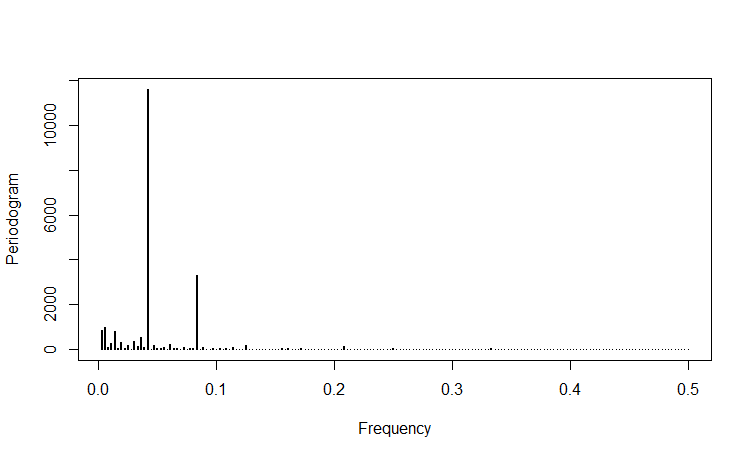
\includegraphics[width=0.8\textwidth]{figures/forecasting/periodogram_July_2014.png}
	\caption{Periodogram of hourly day ahead prices of Nord Pool Spot, Helsinki from July 7th to July 21st in 2014}
	\label{fig:periodogram_July_2014}
\end{figure}

After successfully determine meaningful seasonalities and their resulting periods from the dataset this information can be used to build forecast models that consider the respective seasonal periods in the model generation process. 



\subsection{Seasonal decomposition} \label{ssec:seasonal_decomposition}

Seasonal decomposition describes the process of decomposing a given time series into its components which are trend, seasonal or cyclic and irregular components. Decomposition is done by applying the STL model to the time series and extracting the above mentioned components where STL is defined as Seasonal-Trend decomposition procedure based on Loess \cite{cleveland1990stl}. 

The decomposition of a time series can be formalized as follows \cite{cleveland1990stl}: 

	\[ Y_v = T_v + S_v + R_v \]
	
where $Y_v$ denotes the original time series, $T_v$ the trend component, $S_v$ the seasonal component and $R_v$ the remainder component. $v \in \{ 1,\ldots,N \}$ denotes an individual time stamp in the series where $N$ is the number of unit time stamps in the time series. 

A sample seasonal decomposition of hourly time series is depicted in Figure \ref{fig:stl_decomposition_July_2014}. 

\begin{figure}[htbp]
	\centering
		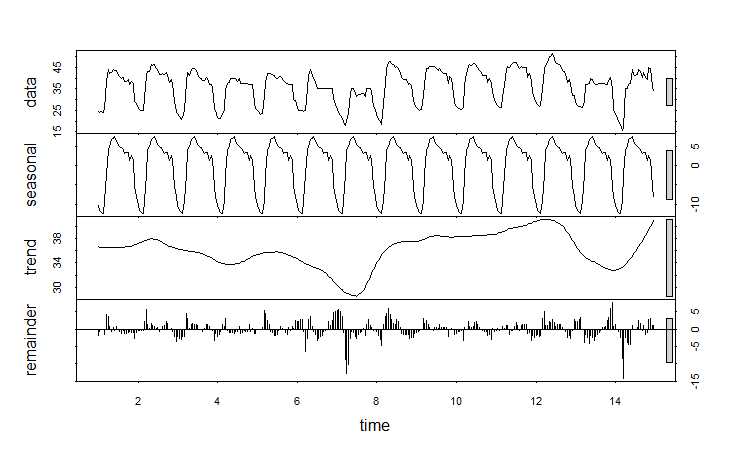
\includegraphics[width=1.00\textwidth]{figures/forecasting/stl_decomposition_July_2014.png}
	\caption{STL decomposition of hourly day ahead time series, Nord Pool Spot, Helsinki from July 7th to July 21st in 2014}	
	\label{fig:stl_decomposition_July_2014}
\end{figure}

The plot consists of four rows with each row containing a different time series component. 
The first row shows the original time series with hourly prices over a time period of two weeks. There are evident daily and weekly seasonal periods visible in the time series. Daily seasonality can be observed by the repetitive pattern of highs and lows over each day whereas weekly seasonality is evident due to the recognizable decline of prices towards the end of each week. 

The second row represents the extracted daily seasonal component which depicts the daily variation in prices. STL is only capable of extracting a single seasonality pattern. In case both daily and weekly seasonal periods should be extracted a BATS or TBATS model can be used (these models are discussed later in this section). 

In the third row the trend component is displayed. It shows a seemingly repetitive pattern over one week, which denotes the weekly seasonal period observable from the original time series. 

Finally in the last row the remaining irregular component is shown which contains all remaining variations in the time series. 

The grey bars at the right hand side of each plot aim to provide a relative comparison of scales over all plots, i.e.~the height of the bars show the same value range in different scales. Thus the whole value range of the trend component is equivalent with the value range of about one third of the original time series. 




\subsection{Forecast models}

Different statistical forecast models have been chosen to be investigated on a large scale. The selection of forecast models includes simpler models such as Simple Exponential Smoothing and more advanced models such as ARIMA and TBATS and variants thereof. The purpose of the evaluation is to provide insights into the performance of different forecast models when applied to electricity price time series. 

\subsubsection{Mean forecast}

The mean forecast is a simple model based on previous observations of a time series. It calculates the mean over a training data set and uses this mean as forecast for all future values \cite{hyndman2012forecasting}. 

It can be formally defined as in equation \ref{eq:mean_forecast}

%\begin{equation}
%\hat{Y}_{t+i} = Y_t
%\label{eq:naive_forecast}
%\end{equation}

\begin{equation}
\hat{y}_{T+h|T} = \frac{1}{T} \sum_{i=1}^T y_i
\label{eq:mean_forecast}
\end{equation}

where $T$ denotes the number of observations in the trainings dataset, $y_i$ denote historical values and $\hat{y}_{T+h|T}$ denotes a forecast of $h$ values into the future beginning at the value of $y_T$. 

Even though the mean forecast only includes simple calculations it can be effective to forecast random or near random time series or time series that exhibit strong volatility. As it is the simplest of the proposed models it should serve as a baseline model to which other models' performance can be compared. 

\subsubsection{Simple Exponential Smoothing}

The Simple Exponential Smoothing model (SES) belongs to the category of exponential smoothing models which calculate the weighted average over historical observations where weights are exponentially decreased for observations in the past. 

As the name implies this model is the simplest of exponential smoothing models which is designed to provide forecast for time series without trend or seasonal components. Similar to the mean forecast model past values of a time series are processed but with given weights that decrease exponentially over time \cite{hyndman2012forecasting,weron2007modeling}. 

The corresponding formula is depicted in Equation \ref{eq:ses_forecast} 

\begin{equation}
\hat{y}_{T+1|T} = \sum_{i=0}^{T-1} \alpha (1 - \alpha)^i y_{T-i}
\label{eq:ses_forecast}
\end{equation}

where $\alpha$ with $0 \le \alpha \le 1$ denotes the smoothing parameter that determines the influence of past observations through setting the corresponding weights. Thus by modifying values of $\alpha$ the resulting impact of past values to forecasted values can be defined. 

\subsubsection{Holt's Exponential Smoothing}

Holt's Exponential Smoothing (Holt's ES) is a linear trend method which extends Simple Exponential Smoothing by including trends in the model generation process \cite{hyndman2012forecasting}. The model consists of two separately modeled components which are level and trend components. These are combined to obtain forecasts for a given time series. It can be formalized by the following equations:

\begin{align}
 \hat{y}_{t+h|t} &= l_t + h b_t \label{eq:holts_forecast} \\
 l_t &= \alpha y_t + (1 - \alpha) (l_{t-1} + b_{t-1})\label{eq:holts_level_component} \\
 b_t &= \beta (l_t - l_{t-1}) + (1 - \beta) b_{t-1}\label{eq:holts_trend_component}
\end{align}

Equation \ref{eq:holts_forecast} denotes the forecast value $\hat{y}_{t+h|t}$ which is forecasted $h$ steps into the future beginning from time stamp $t$. It consists of a combination of the level $l_t$ at time $t$ and the trend $b_t$ at time $t$ continued over the next $h$ time intervals. 

The level component is described in Equation \ref{eq:holts_level_component} which denotes a linear combination of the actual value $y_t$ at time $t$ and the level forecast constructed from previous time stamp's level $l_{t-1}$ and trend $b_{t-1}$ components. 

Equation \ref{eq:holts_trend_component} depicts the trend component which is a linear combination of the difference of the current and previous levels ($l_t, l_{t-1}$) and the estimated trend component $b_{t-1}$ from the previous point in time. 

$\alpha$ and $\beta$ exhibit characteristics $0 \le \alpha \le 1$ and $0 \le \beta \le 1$ and denote the smoothing parameters for the level and trend components, respectively.

\subsubsection{Seasonal HoltWinter's model}

The Seasonal HoltWinter's model is the first of the discussed models which is capable of modeling seasonality in the dataset. It further extends the capabilities of the SES and Holt's ES models by an additional seasonal component. Thus besides the level and trend components $l_t$ and $b_t$ a seasonal component $s_t$ is introduced, with smoothing parameters $\alpha, \beta, \gamma$, respectively \cite{hyndman2012forecasting}. 

The corresponding equations are defined as

\begin{align}
 \hat{y}_{t+h|t} &= l_t + h b_t + s_{t-m+h_m^+} \label{eq:holtwinter_forecast} \\
 l_t &= \alpha (y_t - s_{t-m}) + (1 - \alpha) (l_{t-1} + b_{t-1})\label{eq:holtwinter_forecast_level_component} \\
 b_t &= \beta (l_t - l_{t-1}) + (1 - \beta) b_{t-1}\label{eq:holtwinter_forecast_trend_component} \\
 s_t &= \gamma (y_t - l_{t-1} - b_{t-1}) + (1 - \gamma) s_{t-m}\label{eq:holtwinter_forecast_seasonal_component}
\end{align}

where $m$ denotes the period of seasonality (e.g.~$m=12$ for monthly data when one year is the base unit) and $h_m^+ = \left\lfloor (h-1) \mod m\right\rfloor + 1$ represents the additional number of steps ahead required to model the corresponding seasonal period $m$. Therefore $s_{t-m+h_m^+}$ denotes the previously occurred seasonal period which is added to the forecast equation in Equation \ref{eq:holtwinter_forecast}. 

The level component in Equation \ref{eq:holtwinter_forecast_level_component} is adjusted by the level of the last occurred seasonal period $s_{t-m}$ to consider seasonal differences. The equation for the trend component $b_t$ is taken directly from the one of Holt's ES in Equation \ref{eq:holts_trend_component} whereas the seasonal component is defined in Equation \ref{eq:holtwinter_forecast_seasonal_component}. 

The seasonal component is denoted as a weighted sum of the current value $y_t$ substracted by previous level and trend components and the value of the seasonal component exactly $m$ periods before. 

The smoothing parameters $\alpha, \beta$ and $\gamma$ are estimated by minimizing the squared one-step prediction error to appropriately weigh the different components to yield best results \cite{r2016language}. 


\subsubsection{ARIMA models}

ARIMA models or Auto Regressive Integrated Moving Average models are highly adjustable time series models that can incorporate a number of features from the dataset. They are capable of modeling correlations in the data as well as provide a smoothing method to dampen the impact of extreme outliers. 

ARIMA models may consist of both autoregressive (AR) and moving average (MA) terms to accurately model the underlying dataset \cite{hyndman2012forecasting,weron2007modeling}. 

\paragraph{AR model} The autoregressive component is used to model dependencies in the data such that correlations within the dataset are reduced. It is defined as a weighted sum of past values of an observation. An AR(p) model is shown in Equation \ref{eq:ar_component}.

\begin{equation}
	y_t = c + \sum_{i=1}^p \phi_i y_{t-i} + e_t
\label{eq:ar_component}
\end{equation}

where $y_t$ is modeled as the sum of the past $p$ values of $y$ plus an additional error component $e_t$ and a constant $c$. AR coefficients $\phi_1,\ldots,\phi_p$ are used to weight past observations and need to be estimated in the model generation process. 

\paragraph{MA model} The moving average component models a time series as a moving average of past error terms. Equation \ref{eq:ma_component} gives the formal definition: 

\begin{equation}
	y_t = c + e_t + \sum_{i=1}^q \theta_i e_{t-i}
\label{eq:ma_component}
\end{equation}

where $e_t$ denotes the forecast error at time $t$ and the error terms are weighted by MA coefficients $\theta_1,\ldots,\theta_q$.

\paragraph{ARIMA model} An ARIMA model consist of both AR and MA terms. In addition ARIMA models are able to model non-stationary time series by applying differencing operations to the dataset. ARIMA(p,d,q) denotes a model consisting of $p$ number of AR terms, $q$ MA terms and $d$ number of differences. 
It can be described as the sum of AR and MA terms:

\begin{equation}
	y_t = \sum_{i=1}^p \phi_i y_{t-i} + \sum_{i=1}^q \theta_i e_{t-i} + e_t + c
\label{eq:arima_model}
\end{equation}

When applying the model the possible applied differences during data preprocessing are reversed by integrating the results which refers to the \textit{Integrating} part of the model. 

ARIMA models can be enhanced to model seasonal periods which are defined as ARIMA (p,d,q)(P,D,Q)\textsubscript{m} also denoted as SARIMA models. 
In addition to non-seasonal parameters $p, d$ and $q$ the seasonal parameters $P$, $D$ and $Q$ denote the seasonal AR, differencing and MA components, respectively. 



\subsubsection{BATS and TBATS models}

Multiple seasonal periods can be applied by models such as BATS and TBATS \cite{r2016language}. This can be done by applying a BATS or TBATS model to the time series, identifying different seasonal and trend components and modeling each component separately \cite{de2011forecasting}. 

Both BATS and TBATS models are able to handle multiple seasonalities in the data, i.e.~considering both daily and weekly seasonal periods where TBATS models are capable of modeling non-integer periods as well (e.g.~365.25 for annual seasonality). 

\paragraph{BATS model} BATS stands for Box-Cox transform, ARMA errors, Trend, and Seasonal components. TBATS can then be regarded as the trigonometric version of BATS. 

The definition of BATS is outlined in the following equations: 


\begin{equation}
	y_t^{(\omega)} = 
	\begin{cases}
		\frac{y_t^\omega - 1}{\omega}, & \omega \neq 0 \\
		\log y_t, & \omega = 0
	\end{cases}
\end{equation}


%\begin{equation}
	%y_t^{(\omega)} = 
	%\begin{cases}
		%\frac{y_t^\omega - 1}{\omega}, & \text{if}\ a=1 \\
		%\log y_t, & \text{otherwise}
	%\end{cases}
%\end{equation}


\begin{align}
	y_t^{(\omega)} &= l_{t-1} + \phi b_{t-1} + \sum_{i=1}^T s_{t-m_i}^{(i)} + d_t\label{eq:bats_model} \\
	l_t &= l_{t-1} + \phi b_{t-1} + \alpha d_t \\
	b_t &= (1 - \phi) b + \phi b_{t-1} + \beta d_t \\
	s_t^{(i)} &= s_{t-m_i}^{(i)} + \gamma_i d_t\label{eq:bats_seasonal} \\
	d_t &= \sum_{i=1}^p \Phi_i d_{t-i} + \sum_{i=1}^q \theta_i e_{t-i} + e_t
\end{align}

where $y_t^{(\omega)}$ denotes the Box-Cox transformed value with parameter $\omega$ where $y_t$ is the current value at time $t$ (See also Box-Cox transform in \ref{ssec:box_cox_transformation}). 

$l_t$ describes the level, $b$ denotes the long term trend, $b_t$ represents the trend, $e_t$ is gaussian white noise with zero mean and constant variance and $s_t^{(i)}$ denotes the i-th seasonal component. $\phi$ denotes the damping parameter for the trend and defines the impact of short and long term trends. All of these components are adjusted by a weighted ARMA component $d_t$ and coefficients $\alpha$, $\beta$ and $\gamma$, respectively. 

A BATS model is parameterized by BATS($\omega$,$\phi$,$p$,$q$,$m_1$,\ldots,$m_T$) with the Box-Cox parameter $\omega$, damping parameter $\phi$, ARMA parameters $p$ and $q$ and seasonal periods $m_1,\ldots,m_T$. A double seasonal model (e.g.~daily and weekly) with an AR(1) component can be described as BATS(1,1,1,0,$m_1$,$m_2$) with default Box-Cox and damping parameters. 

\paragraph{TBATS model} As BATS models possibly result in a large number of states and only pure integer seasonal periods may be modeled, the TBATS model has been developed \cite{de2011forecasting}. This model enhances the BATS model with trigonometric expressions:

\begin{align}
	s_t^{(i)} &= \sum_{j=1}^{k_i} s_{j,t}^{(i)}\label{eq:tbats_seasonal} \\
	s_{j,t}^{(i)} &= s_{j,t-1}^{(i)} \cos \lambda_j^{(i)} + s_{j,t-1}^{*(i)} \sin \lambda_j^{(i)} + \gamma_1^{(i)} d_t \\
	s_{j,t}^{*(i)} &= - s_{j,t-1} \sin \lambda_j^{(i)} + s_{j,t-1}^{*(i)} \cos \lambda_j^{(i)} + \gamma_2^{(i)} d_t 
\end{align}

where $s_{j,t}^{(i)}$ describes the stochastic level of the i-th seasonal component and $s_{j,t}^{*(i)}$ represents the stochastic growth in the level of the i-th seasonal component which can be described as the change of value of the seasonal component over a period of time. $k_i$ is the number of harmonics required for the ith seasonal component, $\gamma_1^{(i)}$ and $\gamma_2^{(i)}$ are smoothing parameters and $\lambda_j^{(i)} = \frac{2 \pi j}{m_i}$ the trigonometric parameter which depends on the corresponding seasonal period $m_i$. 

Finally the model can be obtained by replacing $s_t^{(i)}$ in equation \ref{eq:bats_seasonal} by the trigonometric expression in equation \ref{eq:tbats_seasonal} and replacing $s_{t-m_i}^{(i)}$ in equation \ref{eq:bats_model} by $s_{t-1}^{(i)}$. 


\subsection{Box Cox transformation} \label{ssec:box_cox_transformation}

Box cox transformations are used to transform non-normal data to exhibit a normal distribution like behavior \cite{box1964analysis}. Since most statistical time series models (e.g.~ARIMA) require data to have constant variance this technique can be used as a preprocessing step before applying data to forecasting models \cite{nelson1979experience}. 

The formula for box cox transformations is as follows: 


\begin{equation}
	y^{(\lambda)} = 
	\begin{cases}
		\frac{y^\lambda - 1}{\lambda}, & \lambda \neq 0 \\
		\log y, & \lambda = 0
	\end{cases}
	\label{eq:box_cox_transform}
\end{equation}

\begin{equation}
	y^{(\lambda)} = 
	\begin{cases}
		\frac{(y + c)^\lambda - 1}{\lambda}, & \lambda \neq 0 \\
		\log (y + c), & \lambda = 0
	\end{cases}
	\label{eq:box_cox_transform_with_constant}
\end{equation}

where conditions $y > 0$ and $y > -c$ apply to equations \ref{eq:box_cox_transform} and \ref{eq:box_cox_transform_with_constant}, respectively. 

Since the value of $\lambda$ can be less than one $y$ has to be positive and thus a constant term $c > 0$ is required in case $y < 0$ (equation  \ref{eq:box_cox_transform_with_constant}). 

In \cite{nelson1979experience} the autors show that it might not be always possible to transform a series to show a normal distribution and that the application of the procedure can be costly. Still some improvements to forecasts can be achieved by applying Box-Cox transformation to non-normal distributions as a preprocessing step to model generation. 


\subsection{Forecast accuracy measures} \label{ssec:forecast_acc_measures}

Different forecast accuracy methods can be applied to investigate model performance. These methods are based on estimating the overall forecast error for a given model and forecast horizon \cite{hyndman2012forecasting, weron2007modeling}. 

The forecast errors are computed as a function of residuals which are defined as the differences of actual values to forecasts \cite{hyndman2012forecasting}: 

\begin{equation}
	e_i = y_i - \hat{y_i}
\label{eq:residuals}
\end{equation}

where $\hat{y_t}$ denotes the one step ahead forecast based on a series of past values $\{y_1,\ldots,y_{t-1}\}$. 


\subsubsection{Scale-dependent error measures}

Scale dependent errors are absolute error measures depending on the scale of the examined dataset. Therefore when comparing these types of error measures they should be applied to data showing the same scale. 

\paragraph{Mean error}
The mean error (ME) denotes a measure of the mean value of forecast errors over a given period of time. 
It can be seen as indication of the symmetry of the forecast error distribution. 

\begin{equation}
\frac{1}{n} \sum_{i=1}^{n} \hat{y}_i - y_i
\label{eq:acc_me}
\end{equation}

where $n$ is the number of observations, $\hat{y}_i$ is the forecast for observation $i$ and $y_i$ denotes the actual value for observation $i$. 

\paragraph{Mean absolute error}
The mean absolute error (MAE) shows the mean of all absolute errors over the forecast horizon where the absolute error is defined by the absolute difference between a value of the dataset and its forecasted value. The mean absolute error provides a means for retrieving a measure proportional to actual forecast errors. 

\begin{equation}
\frac{1}{n} \sum_{i=1}^{n} |\hat{y}_i - y_i|
\label{eq:acc_mae}
\end{equation}



\paragraph{Root mean squared error}
The root mean squared error (RMSE) takes the root of the sum of the squared forecast errors which puts more emphasis on possible outliers in residual values. 

\begin{equation}
	\sqrt{\frac{1}{n} \sum_{i=1}^{n} (\hat{y}_i - y_i)^2}
\label{eq:acc_rmse}
\end{equation}


\subsubsection{Percentage based error measures}

Percentage based error measures have the advantage of providing scale independent measures for comparing forecast errors across different time series. However a significant disadvantage of percentage errors is their inability to handle zero values in time series. Also numerical compuations become unstable when values get closer to zero. 


\paragraph{Mean percentage error}

The mean percentage error (MPE) is dependent on the symmetry of the forecast error distribution as positive and negative value differences might cancel each other out. This can be compared to the mean error which shows the same behavior as a scale dependent measure. 


\begin{equation}
\frac{1}{n} \sum_{i=1}^{n} \frac{\hat{y}_i - y_i}{y_i}
\label{eq:acc_mpe}
\end{equation}



\paragraph{Mean absolute percentage error}

The mean absolute percentage error (MAPE) shows similar to the mean absolute error the mean of all absolute errors but as percentage error relative to the corresponding actual value. 

\begin{equation}
\frac{1}{n} \sum_{i=1}^{n} \left|\frac{\hat{y}_i - y_i}{y_i}\right|
\label{eq:acc_mape}
\end{equation}




\section{Model generation} \label{sec:model_generation}

In this section the procedure of generating an ARIMA model is described. Since ARIMA models are classical time series models which showed reasonable results in energy price forecasting \cite{aggarwal2009electricity,weron2005forecasting} they have been investigated in detail to provide a better understanding of the model generation process. 

In addition to the well known Box Jenkins approach (see section \ref{ssec:arima_models_to_predict_next_day_prices}) a custom model selection process is proposed for manual ARIMA model selection \cite{hyndman2012forecasting}. This process is outlined in Figure \ref{fig:manual_arima_forecasting_procedure}.

\begin{figure}[htbp]
	\centering
		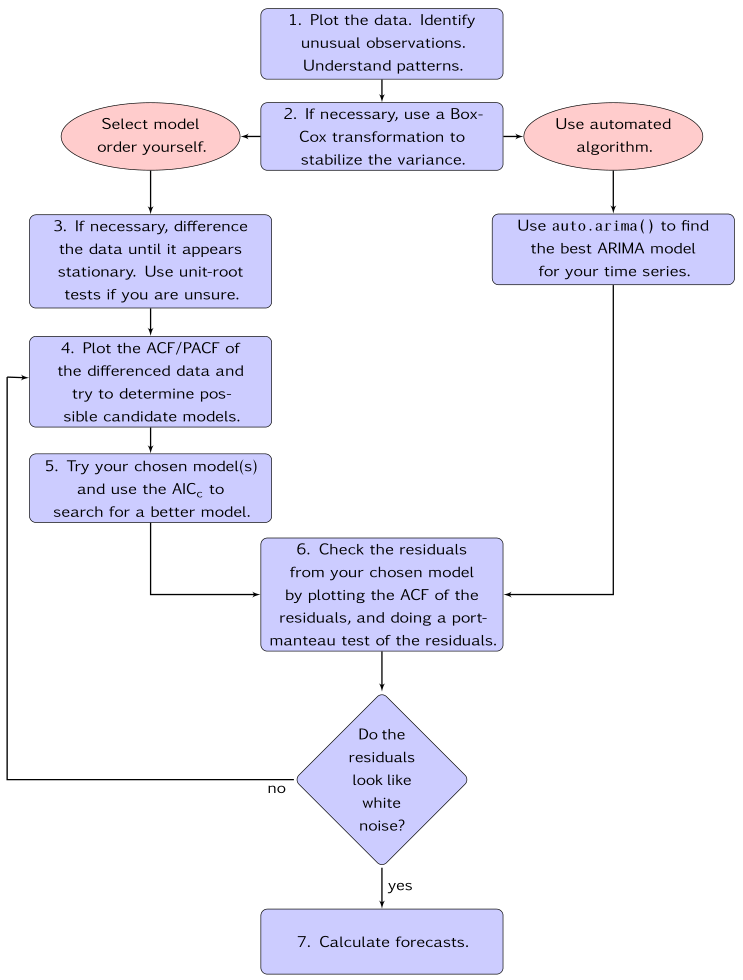
\includegraphics[width=0.70\textwidth]{figures/forecasting/manual_arima_forecasting_procedure.png}
	\caption{Manual ARIMA model generation process \cite{hyndman2012forecasting}}
	\label{fig:manual_arima_forecasting_procedure}
\end{figure}

In this case a manual model generation process is conducted. The data based on which a model will be generated together with diagnostic plots (ACF, PACF) is shown in Figure \ref{fig:tsdiag_prices_acf_pacf}. 

\begin{figure}[htbp]
	\centering
		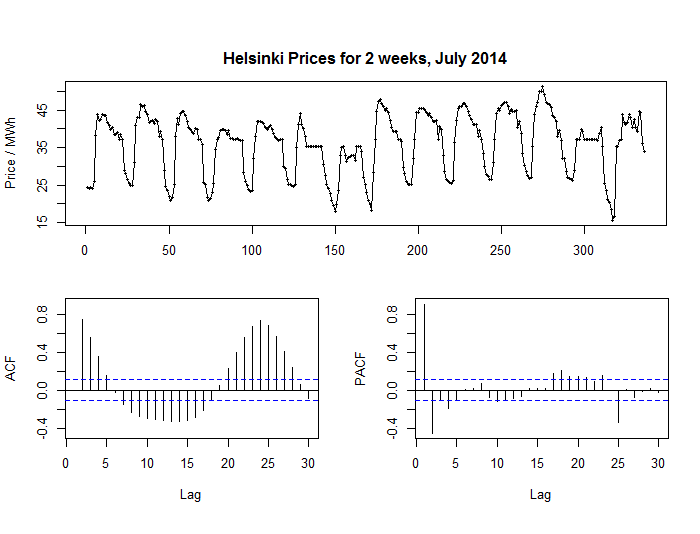
\includegraphics[width=0.95\textwidth]{figures/forecasting/tsdiag_prices_acf_pacf.png}
	\caption{Two weeks of hourly day ahead prices with ACF and PACF plots (Nord Pool Spot, Helsinki from July 7th to July 21st in 2014)}
	\label{fig:tsdiag_prices_acf_pacf}
\end{figure}

The dataset consists of two weeks of hourly day ahead prices amounting to a total of 336 hours. Figure \ref{fig:tsdiag_prices_acf_pacf} shows three plots, at the top a time series plot showing the energy price time series is depicted, on the bottom left an autocorrelation plot (ACF) is shown and on the bottom right a partial autocorrelation plot (PACF) is printed. 
As already discussed in section \ref{ssec:seasonal_decomposition} this data exhibits daily and weekly seasonality which is clearly visible on the time series plot. 

As ARIMA models require data to be stationary (i.e.~it exhibits no trend or seasonality) the proposed method to transform a series into a stationary series is to apply one or more levels of differencing or seasonal differencing. The resulting residuals of the model should show no autocorrelations and should exhibit a zero mean \cite{hyndman2012forecasting}. Ideally residuals have constant variance and exhibit a normal distribution as well. 

ACF and PACF plots are diagnostic plots to examine correlations within the dataset \cite{nist2012handbook,nau2016statistical}. 
Both ACF and PACF plots display individual lags on the x-coordinate while on the y-coordinate the values of the autocorrelation and partial autocorrelation functions are displayed for ACF and PACF plots, respectively. The dashed blue lines denote the 95\% confidence interval for white noise, i.e.~lag values contained within this interval do not reject the white noise hypothesis. 
Values exceeding the confidence bounds are "`significant"' regarding correlations in the data. 
%However 1 in 20 lags is allowed to exceed the significance bounds without violating the white noise assumption. 

The ACF plot displays the ``coefficients of correlation between a time series and lags of itself'' whereas the PACF plot shows the ``partial correlation coefficients between the series and lags of itself'' \cite{nau2016statistical}. 
Correlation coefficients for autocorrelations are said to be interdependent which means that the value of an autocorrelation at lag $h$ depends on correlations of all previous lags $1,\ldots,h-1$. In contrast, partial autocorrelations only include correlations specific to lag $h$ without considering correlations at lower order lags. 

According to the model generation process in Figure \ref{fig:manual_arima_forecasting_procedure} data should be differenced if necessary to make the series stationary. In this case a seasonal difference might be appropriate due to the obvious seasonality in the time series. 

The ACF plot above shows a decay of significant autocorrelations whereas the PACF plot depicts several significant spikes with most significant ones at lags 2 and 25. 
As the spike at lag 25 in the PACF plot is close to the assumed seasonal period of 24 this may suggest adding a seasonal AR(1) term with a period of 24. The peak value at lag 24 in the ACF plot may be another indicator of seasonal correlation.
Therefore, the suggested intermediate ARIMA model is ARIMA(0,0,0)(1,1,0)[24] with a seasonal AR term and one level of seasonal differencing with a period of 24. 

The resulting model residuals are depicted in Figure \ref{fig:residuals_arima_000_110}. 

\begin{figure}[htbp]
	\centering
		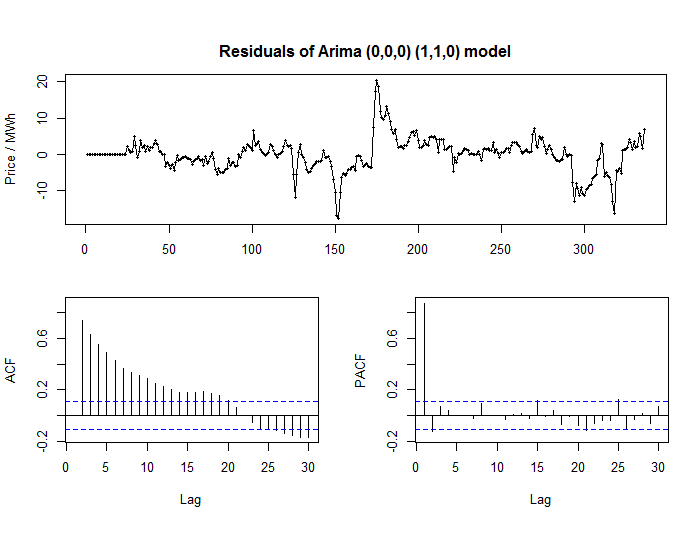
\includegraphics[width=0.95\textwidth]{figures/forecasting/residuals_arima_000_110.png}
	\caption{Intermediate ARIMA(0,0,0)(1,1,0)[24] model with seasonal difference}
	\label{fig:residuals_arima_000_110}
\end{figure}

Figure \ref{fig:residuals_arima_000_110} depicts residuals with removed hourly seasonality and zero mean. However the series can not be regarded as stationary as significant deviations exist from the mean in the time series. Apart from the weekly seasonality further correlations can be identified. 

According to \cite{nau2016statistical} a cut-off (rapid decrease of correlation values) at the PACF plot indicates adding an AR term with an order corresponding to the number of the last significant lag of this occurrence. Conversely a cut-off at the ACF plot indicates the addition of a MA term with the number of the last significant lag in the ACF plot. 

Since Figure \ref{fig:residuals_arima_000_110} shows a slow decay in the ACF and a small but significant coefficient at lag 2 in the PACF we recognize a cut-off at this lag in the PACF and add a (non-seasonal) AR(2) term to the model. 
Thus the resulting model is ARIMA(2,0,0)(1,1,0)[24] which is shown in Figure \ref{fig:residuals_arima_200_110}. 

\begin{figure}[htbp]
	\centering
		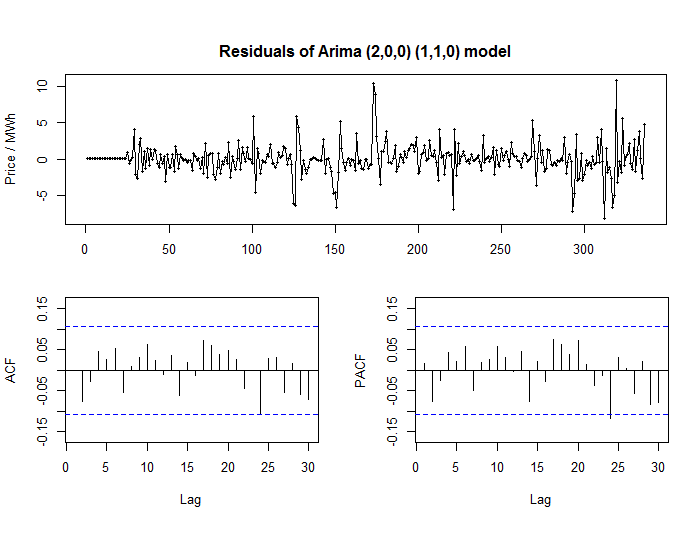
\includegraphics[width=0.95\textwidth]{figures/forecasting/residuals_arima_200_110.png}
	\caption{Residuals of ARIMA(2,0,0)(1,1,0)[24]}
	\label{fig:residuals_arima_200_110}
\end{figure}

The time series of residuals above can be assumed to be stationary as no significant deviations from the mean are visible. 

There is only one significant spike at lag 24 remaining which might indicate still some seasonal information in the data, however it could be as well regarded as outlier as 1 in 20 spikes is said to be significant by chance alone \cite{hyndman2012forecasting}. 


%
%The autocorrelation function determines the existence or non-existence of correlation between lagged variables within a time series \cite{nist2012handbook}. 
%That is, the correlation between a point in the time series to another point in the same time series is calculated where the gap between the two points is fixed by the given lag (hence the name \textit{auto}-correlation). 
%
%The autocorrelation function is defined as the autocorrelation coefficient $R_h$ (equation \ref{eq:autocorr_coeff})
%
%\begin{equation}
%R_h = \frac{C_h}{C_0}
%\label{eq:autocorr_coeff}
%\end{equation}
%
%
%where $C_h$ denotes the autocovariance function and $C_0$ defines the variance function 
%(see equations \ref{eq:autocov_func} and \ref{eq:variance_func}). 
%
%
%\begin{equation}
%C_h = \frac{1}{N} \sum\limits_{t=1}^{N-h} (Y_t - \bar{Y}) (Y_{t+h} - \bar{Y})
%\label{eq:autocov_func}
%\end{equation}
%
%
%\begin{equation}
%C_0 = \frac{1}{N} \sum\limits_{t=1}^{N} (Y_t - \bar{Y})^2
%\label{eq:variance_func}
%\end{equation}
%
%with $\bar{Y}$ denoting the mean of the series, $N$ defines the sample size, $Y_t$ the observation at time $t$ and $Y_{t+h}$ the observation $h$ steps ahead from $t$. 
%The autocovariance function determines the mean of covariance between variables with fixed lag $h$ while the variance function determines the mean variance over all timestamps $N$. 



\subsection{Model validation}



The corrected Akaike Information Criterion (AICc) is a well known goodness of fit measure for stochastic models \cite{weron2007modeling}. It provides a relative quality measure for models such that models with lower AICc values are assumed to better capture the characteristics of the underlying data. 
Equation \ref{eq:aicc_test} defines the metric. 

\begin{equation}
	AICc = -2 \log \mathcal{L} + \frac{2dn}{n - d - 1}
\label{eq:aicc_test}
\end{equation}

with $\log \mathcal{L}$ being the log-likelihood, $d$ the model size (number of parameters) and $n$ denotes the sample size. Note that the model size $d$ is present in order to penalize models having too many parameters. The log-likelihood function estimates how well the model fits the data. 

After a model has been chosen by evaluating the AICc value the model residuals should be checked for existing correlations. As shown in the last section this can be done by verifying the ACF and PACF plots but tests are available for automated testing against randomness \cite{weron2007modeling,hyndman2012forecasting}. 

One of these tests is the Ljung Box test which tests a given number of autocorrelations if they fall outside the significance bounds \cite{weron2007modeling}. The test is defined in Equation \ref{eq:ljung_box_test}. 

%for probability of showing non-white noise properties 
\begin{equation}
	Q = n(n + 2) \sum_{j=1}^{h} \frac{\hat{\rho}^2 (j)}{n - j}
\label{eq:ljung_box_test}
\end{equation}

with $n$ as the sample size, $h$ as number of lags and $\hat{\rho}^2 (j)$ as the squared autocorrelation at lag $j$. 
Its distribution can be approximated by the $\chi^2$ distribution with $h$ degrees of freedom. The white noise hypothesis is rejected if $Q > \chi_{1-\alpha}^2 (h)$ with a defined significance level $\alpha$ with $\chi_{1-\alpha}^2$ being the $(1 - \alpha)$ quantile of the $\chi^2$ distribution with $h$ degrees of freedom. 


\subsection{Model evaluation} \label{ssec:model_evaluation}

In order to assess the quality and goodness of fit of the models generated in section \ref{sec:model_generation} they are validated and compared to a model generated by an automatic model generation procedure. 

In addition to the manual model selection procedure shown in the last section automatic model generation procedures exist to detect the model with best goodness of fit parameters by iterating over a set of candidate models. 

For generating ARIMA models the \textit{auto.arima} function may be used \cite{hyndman2012forecasting,r2016language}. 

It is defined by the following steps \cite{hyndman2012forecasting}: 

\begin{enumerate}
	\item Determine the number of differences $d$ by applying a unit root test (e.g.~KPSS test).
	\item A set of candidate models is generated starting with the following models: 
				
				ARIMA(2,d,2) \\
				ARIMA(0,d,0) \\
				ARIMA(1,d,0) \\
				ARIMA(0,d,1) 
				
				Model parameters $p$ and $q$ are modified by adding $\pm 1$ where the best model is set as reference. 
				Repeat the last line until no model with a lower AICc value can be found. 

\end{enumerate}

A model has been generated using auto.arima based on the same data as used for manual model selection in section \ref{sec:model_generation}. 
The resulting models with corresponding model parameters are outlined in table \ref{tab:model_names_and_parameters}. 

\begin{table}[ht]
\centering
\begin{tabular}{l|l}
 Model Name & Model Parameters \\ 
  \hline
	Intermediate Model	& ARIMA(0,0,0)(1,1,0)[24] \\ 
	Final Model 				& ARIMA(2,0,0)(1,1,0)[24] \\ 
	Automatic Model 		& ARIMA(2,0,3)(1,0,2)[24] \\ 
\end{tabular}
\caption{Model names and parameters}
\label{tab:model_names_and_parameters}
\end{table}

AICc and Ljung Box values have been calculated for each model defined above. For Ljung Box tests a 95\% confidence interval has been used
such that resulting p-values greater than 0.05 indicate white noise properties of the residuals. Thus a high Ljung Box test value gives 
high probability of a series resembling white noise. 

The AICc and Ljung Box values are outlined in table \ref{tab:model_aicc_and_ljung_box_values}. 

\begin{table}[ht]
\centering
\begin{tabular}{r|r|r|r}
 & Intermediate Model & Final Model & Automatic Model \\ 
  \hline
	AICc 			& 1868.01 & \textbf{1400.22} & 1457.26 \\ 
  Ljung Box & < 2.2e-16 & 0.1523 & \textbf{0.9927} \\ 
\end{tabular}
\caption{AICc and Ljung Box values}
\label{tab:model_aicc_and_ljung_box_values}
\end{table}

Results show that it is possible for manually selected models to outperform automatically generated models, i.e.~the Final Model shows a lower AICc value than the Automatic Model. This is presumably due to the manual model using explicit seasonal differencing which the automatic nodel does not use. However the Ljung Box test values indicate a different result where the Automatic Model results in a higher p-value and thus exhibits less correlations than the Final Model. As both models exceed the significance bounds of 0.05 this is only of minor importance as both exhibit white noise characteristics. If in doubt the AICc value should be given precedence over Ljung Box test results. 

\section{Model selection algorithm} \label{sec:model_selection_algorithm}

An automated model selection algorithm has been implemented to provide aid in finding suitable ARIMA models for a given trainings dataset. 
The process consists of several data preprocessing steps with generation and comparison of different ARIMA models and model evaluation based on a weighted function of AICc and Ljung Box test values. 

The model selection algorithm consists of three separate functions each contributing a different part to model generation. These functions are \textit{GenerateArimaModel} as the base function for model generation, \textit{AutomatedBoxTest} for determining the right parameters for the Ljung Box tests and \textit{SeasonalPeriods} for estimation of possibly existing seasonal periods within the data. 

%They will be referred to each other as soon as they are called. 

\subsection{Function GenerateArimaModel}

\begin{enumerate}
	\item Get trainingsdata
	
	\begin{enumerate}
		\item Read time series of energy prices from given location
		\item Define trainings period by start and end date
	\end{enumerate}
	\item Determine seasonality
	
	\begin{enumerate}
		\item Call \textit{SeaonalPeriods} to retrieve seasonal periods from the data
	\end{enumerate}
	
	\item Create time series objects
	
	\begin{enumerate}
		\item For each seasonal period found create a time series object based on that period
	\end{enumerate}
	
	\item Calculate the Box-Cox transformation parameters
	
	\begin{enumerate}
		\item Compute the Box Cox parameters for each of the created time series objects
	\end{enumerate}
	
	\item Create models
	
	\begin{enumerate}
		\item Create model(s) without BoxCox transformation
		
		\begin{enumerate}
			\item Generate model with auto.arima for each of the created time series objects 
		\end{enumerate}
		
		\item Create model(s) with BoxCox transformation
		
		\begin{enumerate}
			\item Generate model with auto.arima and previously defined lambda (Box-Cox) parameter for each of the created time series objects if Box-Cox parameter is not equal to 1 (then it would have no effect)
		
		\end{enumerate}
		
	\end{enumerate}
	
	\item Execute Ljung Box test for each of the models
	
	\begin{enumerate}
		\item Call \textit{AutomatedBoxTest} to retrieve the Ljung Box p-values for each model
	\end{enumerate}
	
	\item Saving models, boxtests, AICc values and p-values in vectors
	
	\item Model Evaluation

	\begin{enumerate}
		
		\item Check model goodness of fit via AICc value comparison
		
		\begin{enumerate}
			\item $p_{aicc_i} = \frac{1}{| AIC_{min} - AIC_i | + 2}$
			%\item p_aicc = 1 / (abs(AICmin – AIC(i)) + 2)
			\item ``+2'' -> moderate the decrease of values due to the inverse function
		\end{enumerate}
		
		\item Compare p-values of Ljung Box tests to check residual characteristics
		
		\begin{enumerate}
			\item p-values range from 0 to 1 -> determine difference in relation to full range
			\item $p_{ljung} = \frac{p_{value} - 0.05}{1 - 0.05}$
		\end{enumerate}
		
	\end{enumerate}

	\item Model selection

	\begin{enumerate}
		\item Calculate weighted result based on goodness of fit values with user defined weights
		\item $F_i = w_{aicc_i} p_{aicc_i} + w_{ljung_i} p_{ljung_i}$ for each model $i \in M$
	\end{enumerate}
	
	\item Return model with the highest goodness of fit value $F_i$

\end{enumerate}


\subsection{SeasonalPeriods}

	\begin{enumerate}
		\item If target period is specified and enforced
		
		\begin{enumerate}
			\item return a list of (targetPeriod, defaultPeriod) 
		\end{enumerate}
		
		\item Else 
		
		\begin{enumerate}
			\item Get the x most frequent periods sorted by number of occurrences descending, where x is a user defined number (apply periodogram)
			\item If a max period limit has been specified, discard any periods above this limit
			\item If the number of occurrences of a period falls below the white noise threshold, discard the period
			
			\item If the target period is specified and has been found
			
			\begin{enumerate}
				\item return a list of (targetPeriod, defaultPeriod) 
			\end{enumerate}
			
			\item Otherwise
			
			\begin{enumerate}
				\item add the defaultPeriod (=1) to the list of periods and return the list
			\end{enumerate}
		\end{enumerate}
	\end{enumerate}


\subsection{AutomatedBoxTest}

\begin{enumerate}
	\item Determine the most suitable value for the lag based on the sample size and 
	whether seasonal periods are existing in the dataset. 
	
	\begin{enumerate}
		\item The following rules of thumb have been established to determine a suitable value for the lag of the test \cite{hyndman2014blog}: 
		
		\begin{enumerate}
			\item for non-seasonal time series a lag value of $h=min(10,T/5)$ should be used
			\item for seasonal time series a lag value of $h=min(2m,T/5)$ should be used,
				where $T$ denotes the sample size and $m$ the seasonal period
		\end{enumerate}
		
		\item The number of determined lags is reduced by the number of parameters in the model
		
		\item The box test is executed and result is returned
	\end{enumerate}
	
\end{enumerate}


\subsection{Discussion}

The core of the model selection algorithm are steps 8 and 9 of Function GenerateArimaModel where relative measures for both AICc and Ljung Box values have been developed to be able to integrate them into a weighted function. Thus it is possible to define weights to define the impact of each validation measure on forecast model selection. 
As mentionend before (Section \ref{ssec:model_evaluation}) AICc value results should in general be given precedence over Ljung Box values since AICc values are considered more stable. 

Another thing to note is the so called \textit{target period} in function \textit{SeasonalPeriods}. This is a user estimated period which is assumed to be contained in the dataset. If it is found it is given precedence over other periods returned. There is also the possibility of ``enforcing'' the period in which case it is taken without calculating other periods. 





\section{R / Java Simulation Framework}

The R / Java Simulation Framework is responsible for preparation and execution of a large scale simulation of generating and evaluating forecast models over an extended period of time. In this section the architecture and implementation of the simulation framework is presented as well as the interfaces existing between R and Java. 


\subsection{Architecture of the simulation framework}

The framework consists of a Java application server connected to a separately running R server on which R commands are executed. R is a statistical program which is able to model complex statistical functions and includes a considerable amount of statistical packages \cite{r2016project}. It became the de-facto standard for stochastic processing and is available free of charge as well as for various platforms. 

The Java application server has been set up as WildFly 8 \cite{red2016wildfly} with Java Enterprise Edition 7 \cite{oracle2016java} and an Oracle Database \cite{oracle2016database} which provides a scalable architecture including the possibility for modeling web service interfaces. 

In this work a collection of web services has been set up for simple access of data for external applications. This can be used e.g.~by the cloud simulator outlined in section \ref{sec:architecture_of_simulation_framework}. The Java application server wraps methods for retrieval and storage of energy price data, forecast model generation and large scale simulations. It utilizes R for complex statistical processing which is included into advanced methods for simulations and model generation. 

\subsubsection{Class diagram}

In order to visualize the most important entities of the framework a class diagram is outlined in Figure \ref{fig:EPMA_class_diagram}.

A basic entity for energy price retrieval is the \textit{Resource} which wraps the retrieved contents of an energy price source. Data retrieval happens over a generic \textit{DataFetch} interface which is able to fetch data from an URL (e.g.~web service) or directly from a file. The parsing of the energy price data is achieved by a generic \textit{Parser} interface which can be implemented by Parsers for different file types (currently XLS and CSV). 

A \textit{ResourceType} stores a reference to a specific DataFetch and Parser implementation. As source types and formats of energy data will be different for each energy market at least one DataFetch and Parser implementation has to be provided for each market. The \textit{ResourceManager} keeps track of all resources associated with a registered energy market. It is implemented by resource managers for day ahead and real time markets, respectively. 

The \textit{MarketData} entity handles all the logic necessary for actually retrieving energy price data for a given Resource. It provides methods to retrieve data from registered energy sources and subsequently parsing and importing the data into the database. Instances of MarketData are used by \textit{RTPricesResourceRESTService} and \textit{DAPricesResourceRESTService} that provide web service interfaces for data retrieval. In turn, \textit{RManagerResourceRESTService} utilizes these web services to retrieve energy price data for model generation and forecast simulations. 

\begin{figure}[htbp]
	% used to position the image at the horizontal center of the page
	\hspace*{0.5in}
		% include the graphic rotated by a 90 degree angle and scale to paperwidth and height
		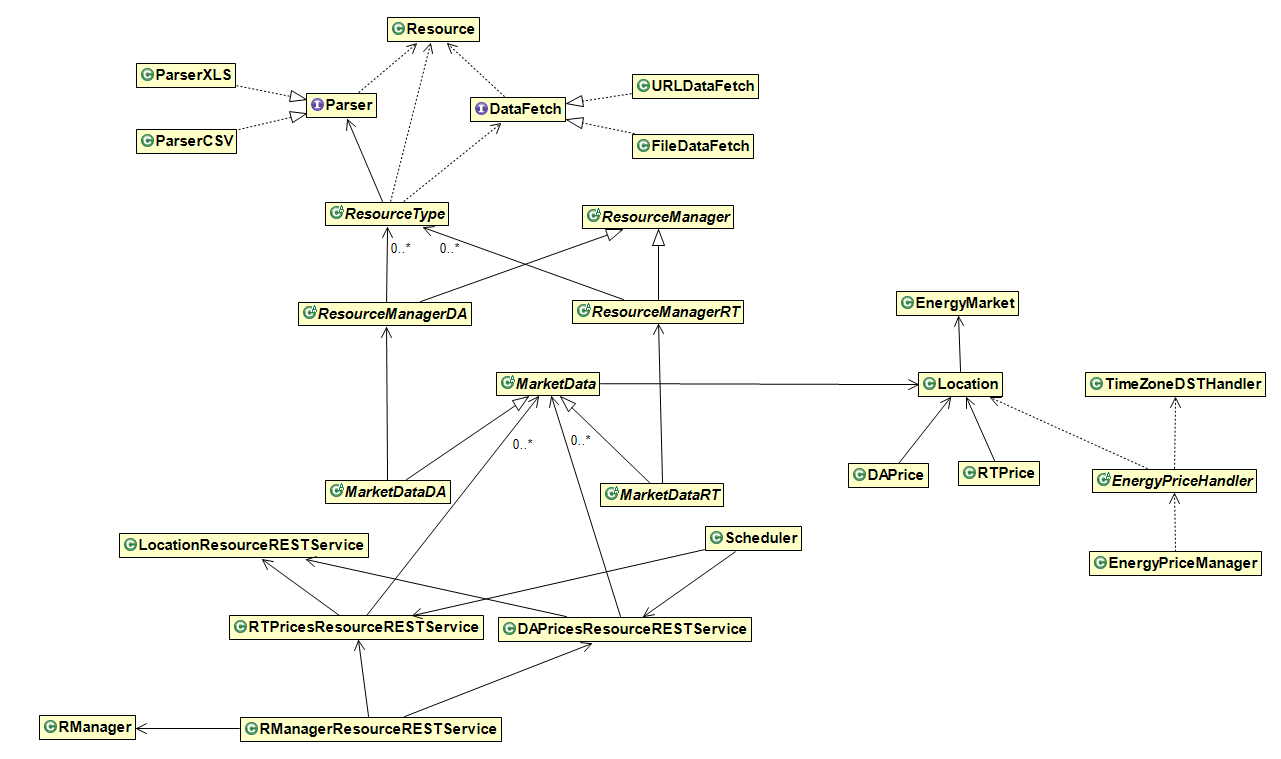
\includegraphics[angle=90,width=\paperheight,height=\paperwidth,keepaspectratio=true]{figures/forecasting/EPMA_class_diagram.png}
	\caption{Class diagram of Energy Price Management Application}
	\label{fig:EPMA_class_diagram}
\end{figure}

The \textit{Scheduler} utilizes Java EE scheduling mechanisms to automatically retrieve energy prices from specific locations at defined time intervals (e.g.~each day at 3 pm). Thus for continuous operation a scheduler can be set up for a location and dates when data should be retrieved regularly from defined interfaces. 

Each MarketData instance stores a reference to a specific \textit{Location} of an \textit{EnergyMarket}. Instances of \textit{DAPrice} and \textit{RTPrice} reference the location from which they were retrieved where these price entities each resemble exactly one energy price entity stored in the database.

Finally the \textit{EnergyPriceHandler} provides a generic interface for parsing energy prices with location specific DST (daylight saving time) changes. This interface is extended by specific implementations of energy markets to manage DST dates. The \textit{TimeZoneDSTHandler} provides a method to retrieve exact DST dates for each location and year. Thus energy prices are stored with dates correctly considering DST changes specific to each location. 

\subsubsection{Web Service interfaces}

The \textit{Energy Price Management Application} (EPMA) on the application server provides different types of web service interfaces. 

Web services are grouped by type: 
%i.e.~management of day ahead prices, real time prices, locations, energy markets and R resources corresponding to classes 

\begin{itemize}
	\item \textit{DAPricesResourceRESTService} for managing day ahead prices
	\item \textit{RTPricesResourceRESTService} for managing real time prices
	\item \textit{LocationResourceRESTService} for managing locations
	\item \textit{EnergyMarketResourceRESTService} for managing energy markets
	\item \textit{RManagerResourceRESTService} for managing R resources
\end{itemize}

Each web service interface is defined by a base path (e.g.~/rtprices), the respective web service name (e.g.~/importall) and mandatory or optional web service parameters. 

%idea: list of all web service methods in the appendix
%
%provide tables with following structure: 
%basepath	web service name		mandatory parameters			optional parameters


%\subsubsection{Energy price data retrieval}



\subsection{R Forecast evaluation}

%fcHorizons <- c("1h","3h","6h","12h","18h","24h","36h","48h","96h","168h")
%accMeasures <- c("ME","RMSE","MAE","MPE","MAPE")
%modelNames <- c("mean","ses","holts","holtwinters","arima","tbats")

The forecast model evaluation discussed in Section \ref{sec:forecast_model_evaluation} is based on implementation of an R function which is called and processed by respective methods on the application server. 

The corresponding R function is named \textit{evaluateModels} and takes energy price data as input separated into a trainings and test data sets. It generates different forecast models based on the given trainings set considering possible seasonal periods in the data (see Section \ref{sec:model_selection_algorithm}) and returns aggregated accuracy measures for each model and forecast horizon. 

\subsubsection{Function evaluateModels}

\begin{tabular}{ll}
\textbf{Input:}  & \textit{pricesTraining} - a list of energy prices taken as trainings data set \\
								 & \textit{pricesTest} - a list of energy prices taken as test data set \\
\textbf{Output:} & \textit{modelList} - a list of models generated within the function \\
								 & \textit{accuracyList} - a list of accuracy measures calculated for each model
\end{tabular}


\begin{lstlisting}[language=R, caption=Function evaluateModels, label={lst:evaluateModelsR}]
evaluateModels <- function(pricesTraining, pricesTest)
{
  period <- getSeasonalPeriod()
  pricesTrainingTs <- generateTimeSeries(pricesTraining, period)
  modelList <- generateModels(Mean,Ses,Holt,HoltWinters, 
	                              Arima,Tbats)						
  accuracyList <- list()
  forecastHorizonList <- (1,3,6,12,18,24,36,48,96,168)
  for( m in modelList ) {
    for( h in forecastHorizonList ) {
      fc <- getForecastForHorizon(m,h)
      accuracyList(m,h) <- getAccuracyMeasures(fc,pricesTest)
    }
  }
  return list(modelList,accuracyList)
}
\end{lstlisting}

In Listing \ref{lst:evaluateModelsR} the function \textit{evaluateModels} is defined. In lines 3 and 4 the most prevailing seasonal period (if any) is determined and 
a time series object is generated based on that period. In line 5 a series of forecast models is generated that are investigated in the algorithm which are Mean forecast model, SES model, Holt (SES with trend), HoltWinters (SES with trend and seasonality), ARIMA (model generation described in Section \ref{sec:model_generation}) and TBATS (seasonal model). 

Line 8 sets a list of forecast horizons in hours, i.e.~forecasts are generated for horizons from 1 up to 168 hours. In line 11 forecasts are produced for each model and forecast horizon separately and in line 12 the generated forecasts are validated by getting accuracy measures for out-of-sample forecasts based on the test data set. 
Line 15 returns a compound object of the list of generated models and accuracy measures. 



\subsection{Java implementation on application server} \label{ssec:java_implementation_on_application_server}

A large scale evaluation of forecasting methods should be conducted where models and corresponding accuracy measures are generated for different training data sets over an extended period of time. 
Thus the application server implements methods for performing customizable forecasting simulations. 

A java method \textit{evaluateModels} in class \textit{RManager} has been implemented which calls the previously introduced R function \textit{evaluateModels} (Listing \ref{lst:evaluateModelsR}) and saves the result in an internal folder on the application server. 
This method is in turn called by an identically named method in \textit{RManagerResourceRESTService} which provides the REST service interfaces to external applications for retrieval of results. 

In order to conduct automated large scale simulations additional methods have been implemented in \textit{RManagerResourceRESTService} to perform customizable simulations. The method \textit{runSimulation} performs a simulation based on a number of parameters. The method signature is depicted in Listing \ref{lst:runSimulation}. 

\begin{minipage}{\linewidth}
\begin{lstlisting}[language=Java, caption=Method runSimulation, label={lst:runSimulation}]
runSimulation(String priceType, Long locationId, 
              String simulationStart, String simulationEnd,
              String trainingsPeriod, String testPeriod, String intervalPeriod)
\end{lstlisting}
\end{minipage}

The \textit{priceType} defines whether the simulation should be based on day ahead or real time prices. Accordingly the parameter is set to either ``da'' or ``rt''. The \textit{locationId} expects an Id of a registered location within the application server. The parameter \textit{simulationStart} expects a date time String containing the start date from where the simulation should be started. The parameter \textit{simulationEnd} describes the end date of the simulation as a date time String, respectively. \textit{trainingsPeriod} is the trainings period for which energy prices should be loaded for model generation, \textit{testPeriod} is the test period against which the models are to be tested and \textit{intervalPeriod} denotes the time interval the simulation should be advanced in each step. 

The corresponding web service interface is given in Listing \ref{lst:runSimulationWebService}. 

\begin{minipage}{\linewidth}
\begin{lstlisting}[language=Java, caption=Method runSimulation web service interface, label={lst:runSimulationWebService}]
/r/simulation/{type}/{loc_id}/{simulationStart}/{simulationEnd}/
                {trainingsPeriod}/{testPeriod}/{intervalPeriod}
\end{lstlisting}
\end{minipage}

The base path of the web service interface is \textit{/r} which is an indicator for web services that are based on R implementations. The name of the web service is \textit{simulation} and parameters have already been described for Listing \ref{lst:runSimulation}. This method or interface is responsible for executing a single simulation with defined start and end dates, trainings-, test- and interval periods. 

A common format has been defined to distinguish different periods and intervals. A regular expression for the format could be described as \textit{\textasciicircum\textbackslash d+[hdw]\$}
which is a combination of at least one digit and one of \textit{h}, \textit{d} or \textit{w} which means \textit{hour}, \textit{day} and \textit{week}, respectively. 
Therefore a trainings period of 2w, 1d or 48h means two weeks, one day or 48 hours. The same holds true for test- and interval periods. 

The method \textit{runSimulation} calls the method \textit{evaluateModels} which performs a single model evaluation for a given trainings and test period. Its method signature is depicted in Listing \ref{lst:evaluateModels}. 

\begin{minipage}{\linewidth}
\begin{lstlisting}[language=Java, caption=Method evaluateModels, label={lst:evaluateModels}]
evaluateModels(String simulationName, String priceType, Long locationId, 
              String startTraining, String endTraining,
              String startTest, String endTest)
\end{lstlisting}
\end{minipage}

This method is responsible for conducting a model evaluation by calling the respective same-named function on the \textit{RManager}. This method is called for each simulation run triggered by the \textit{runSimulation} method, i.e.~it is called for different trainings-, test- and interval periods. In order to distinguish different simulations where each simulation is saved in a folder named after the simulation name the simulationName has been normed (Listing \ref{lst:simulationName_definition}): 

\begin{minipage}{\linewidth}
\begin{lstlisting}[caption=Definition of the simulation name, label={lst:simulationName_definition}]
Definition of the simulation name: 
	
<priceType>_sim_<locationId>_<trainingsPeriod>_<testPeriod>_<intervalPeriod>
\end{lstlisting}
\end{minipage}

where \textit{priceType} is the type of energy price (``da'' or ``rt''), \textit{sim} is a delimiter common to all simulations, \textit{locationId} is the id of the location for which to conduct the simulation, \textit{trainingsPeriod} is the encoded form of the trainings period, the same holds true for \textit{testPeriod} and \textit{intervalPeriod}. All parameters are delimited by underscores to clearly distinguish different parameters. 

Therefore a valid simulation name would be \textit{da\_sim\_1\_2w\_1w\_1w} denoting a simulation on day ahead prices for location with Id 1, 2 weeks trainings period, 1 week test period and 1 week interval period. 

The method \textit{runSimulation} calls the method \textit{evaluateModels} repeatedly over the whole simulation time period (simulation start to simulation end) in intervals specified by the \textit{intervalPeriod} with trainings and test periods specified by the \textit{trainingsPeriod} and \textit{testPeriod} parameters. 

The results of each call of evaluateModels are saved in a separate file under a folder named the same as the simulation. Each file has a naming convention of \textit{<simulationName>\_<start\\Training>} where \textit{startTraining} denotes the start date of the trainings period for this simulation. 



\section{Forecast model evaluation} \label{sec:forecast_model_evaluation}

A large scale forecast model evaluation is performed over an extended period of time in order to identify models that show good performance across different sets of energy price time series. Different metrics and forecast horizons are investigated for a thorough evaluation of model performance to derive the best model from the simulations. 

Four simulations have been run based on data from four different energy markets, namely \textit{Nord Pool Spot}, \textit{Belpex}, \textit{ISO New England} and \textit{PJM}. A time period of three years of energy price data has been chosen to be able to make a meaningful statement about forecast performance on energy prices. 

For each of these locations three different training periods have been evaluated: two weeks, three weeks and four weeks. The simulations have been run with intervals of 1 week. The (maximum) test period has been set to 1 week as well. 

The resulting simulations according to the defined format in Section \ref{ssec:java_implementation_on_application_server} are outlined in Table \ref{tab:list_of_conducted_forecast_simulations}. Each of these simulations and models are evaluated for five different accuracy measures to get a broader view of the model performances (see also Section \ref{ssec:forecast_acc_measures}): 

\begin{itemize}
	\item Mean error (ME)
	\item Mean absolute error (MAE)
	\item Root mean squared error (RMSE)
	\item Mean percentage error (MPE)
	\item Mean absolute percentage error (MAPE)
\end{itemize}

In addition, each of these error measures has been evaluated for ten different forecast horizons (in hours): 
1, 3, 6, 12, 18, 24, 36, 48, 96, 168. Thus one goal of the simulations is to evaluate the performance of models when exposed to 
different forecast horizons. 

\begin{table}[ht]
\centering
\begin{tabular}{llllll}
  \hline
 Simulation Name &  Type & Location & Trainings Period & Test Period & Interval Period \\
  \hline
	da\_sim\_1\_2w\_1w\_1w & day ahead & Hamina & 2 weeks & 1 week & 1 week \\
	da\_sim\_1\_3w\_1w\_1w & day ahead & Hamina & 3 weeks & 1 week & 1 week \\
	da\_sim\_1\_4w\_1w\_1w & day ahead & Hamina & 4 weeks & 1 week & 1 week \\
	\hline
	da\_sim\_2\_2w\_1w\_1w & day ahead & St.Ghislain & 2 weeks & 1 week & 1 week \\
	da\_sim\_2\_3w\_1w\_1w & day ahead & St.Ghislain & 3 weeks & 1 week & 1 week \\
	da\_sim\_2\_4w\_1w\_1w & day ahead & St.Ghislain & 4 weeks & 1 week & 1 week \\
	\hline
	rt\_sim\_4\_2w\_1w\_1w & real time & Portland & 2 weeks & 1 week & 1 week \\
	rt\_sim\_4\_3w\_1w\_1w & real time & Portland & 3 weeks & 1 week & 1 week \\
	rt\_sim\_4\_4w\_1w\_1w & real time & Portland & 4 weeks & 1 week & 1 week \\
	\hline
	rt\_sim\_6\_2w\_1w\_1w & real time & Richmond & 2 weeks & 1 week & 1 week \\
	rt\_sim\_6\_3w\_1w\_1w & real time & Richmond & 3 weeks & 1 week & 1 week \\
	rt\_sim\_6\_4w\_1w\_1w & real time & Richmond & 4 weeks & 1 week & 1 week \\
   \hline
\end{tabular}
\caption{List of all conducted forecast simulations}
\label{tab:list_of_conducted_forecast_simulations}
\end{table}




\subsection{Forecast evaluation results}

For conducting the simulations energy price data has been taken from years 2012 to 2014. As mentioned above model evaluations have been done in intervals of 1 week and forecast errors have been measured based on different trainings and test data sets for various forecast horizons. Each of the forecast error results has been aggregated for the respective trainings-, test period and forecast horizon over the whole time period of the simulation. 


\subsubsection{Result tables} \label{sssec:result_tables}

Aggregated RMSE results for Hamina belonging to the Nord Pool Spot power market are shown in Tables \ref{tab:results_hamina_2weeks}, \ref{tab:results_hamina_3weeks} and \ref{tab:results_hamina_4weeks} for 2, 3 and 4 weeks of trainingsdata, respectively. 


%> batchRMSEResults(1)
% latex table generated in R 3.1.1 by xtable 1.8-2 package
% Fri Mar 25 18:58:38 2016
\begin{table}[ht]
\centering
\begin{tabular}{rrrrrrrrrrr}
  \hline
 & 1h & 3h & 6h & 12h & 18h & 24h & 36h & 48h & 96h & 168h \\ 
  \hline
mean & 9.30 & 10.66 & 10.79 & 14.78 & 14.22 & 13.02 & 13.21 & 12.58 & 12.99 & 12.18 \\ 
  ses & 2.13 & 3.54 & 5.06 & 15.83 & 16.38 & 14.98 & 14.97 & 14.64 & 15.13 & 13.30 \\ 
  holts & 1.91 & 3.36 & 9.48 & 30.83 & 38.85 & 44.08 & 58.79 & 74.25 & 137.44 & 228.66 \\ 
  holtwinters & 3.22 & 7.15 & 13.18 & 26.22 & 36.32 & 46.07 & 65.31 & 85.66 & 167.14 & 289.51 \\ 
  arima & 2.11 & 3.08 & 4.65 & 13.66 & 13.89 & 12.67 & 12.87 & 12.61 & 13.68 & 12.98 \\ 
  tbats & 2.16 & 2.89 & 4.35 & 10.68 & 10.89 & 10.02 & 10.19 & 9.94 & 10.70 & 10.33 \\ 
   \hline
\end{tabular}
\caption{Forecast evaluation results based on RMSE for a trainings period of 2 weeks, Nord Pool Spot, Hamina}
\label{tab:results_hamina_2weeks}
\end{table}
% latex table generated in R 3.1.1 by xtable 1.8-2 package
% Fri Mar 25 18:58:38 2016
\begin{table}[ht]
\centering
\begin{tabular}{rrrrrrrrrrr}
  \hline
 & 1h & 3h & 6h & 12h & 18h & 24h & 36h & 48h & 96h & 168h \\ 
  \hline
mean & 9.40 & 10.75 & 10.90 & 15.03 & 14.46 & 13.25 & 13.44 & 12.81 & 13.27 & 12.42 \\ 
  ses & 2.14 & 3.56 & 5.06 & 15.84 & 16.38 & 14.98 & 14.97 & 14.63 & 15.14 & 13.31 \\ 
  holts & 1.91 & 3.38 & 9.51 & 30.88 & 38.90 & 44.15 & 58.90 & 74.39 & 137.77 & 229.23 \\ 
  holtwinters & 3.44 & 7.61 & 14.06 & 27.95 & 38.22 & 47.77 & 67.07 & 87.51 & 169.44 & 292.43 \\ 
  arima & 2.12 & 2.95 & 4.37 & 13.02 & 13.12 & 11.89 & 11.99 & 11.63 & 12.37 & 11.50 \\ 
  tbats & 2.15 & 3.04 & 4.73 & 11.23 & 11.41 & 10.51 & 10.57 & 10.33 & 11.05 & 10.67 \\ 
   \hline
\end{tabular}
\caption{Forecast evaluation results based on RMSE for a trainings period of 3 weeks, Nord Pool Spot, Hamina}
\label{tab:results_hamina_3weeks}
\end{table}
% latex table generated in R 3.1.1 by xtable 1.8-2 package
% Fri Mar 25 18:58:38 2016
\begin{table}[ht]
\centering
\begin{tabular}{rrrrrrrrrrr}
  \hline
 & 1h & 3h & 6h & 12h & 18h & 24h & 36h & 48h & 96h & 168h \\ 
  \hline
mean & 9.52 & 10.88 & 11.04 & 15.22 & 14.63 & 13.42 & 13.58 & 12.94 & 13.41 & 12.57 \\ 
  ses & 2.13 & 3.57 & 5.06 & 15.84 & 16.38 & 14.97 & 14.96 & 14.61 & 15.13 & 13.30 \\ 
  holts & 1.89 & 3.37 & 9.53 & 31.00 & 39.07 & 44.34 & 59.18 & 74.75 & 138.54 & 230.59 \\ 
  holtwinters & 5.58 & 11.05 & 17.33 & 33.52 & 44.92 & 54.87 & 76.25 & 98.63 & 189.26 & 327.09 \\ 
  arima & 1.98 & 2.85 & 4.39 & 12.69 & 12.79 & 11.60 & 11.73 & 11.35 & 12.06 & 11.12 \\ 
  tbats & 2.20 & 3.09 & 4.64 & 10.98 & 11.19 & 10.31 & 10.45 & 10.20 & 10.91 & 10.36 \\ 
   \hline
\end{tabular}
\caption{Forecast evaluation results based on RMSE for a trainings period of 4 weeks, Nord Pool Spot, Hamina}
\label{tab:results_hamina_4weeks}
\end{table}


Results show that forecasts over different horizons exhibit comparable relative values across almost all forecasting models. That is, values behave in a similar way across forecast models when examining different forecast horizons. 

Notably values stay much in the same value range except for Holts and HoltWinters models where forecast errors increase non-linearly with an increase of forecast horizon. This may be due to their inability to capture short term seasonality. 

From the results it is visible that the forecast periods from 24 hours to 48 hours provide the best results through almost all models. A forecast period of 48 hours seems to provide the best results apart from results for low periods (1 to 6 hours). Small forecast horizons generally exhibit smaller forecast errors as the short period of time does not allow a high value for aggregated deviations from the series. Therefore it can be stated that forecast error results can only be meaningfully compared among forecast windows of a minimum of 12 hours. 

When comparing performance of forecast models the TBATS model clearly exhibits the lowest forecast errors when considering forecast windows from 12 hours upwards. It is followed by the ARIMA model and, suprisingly by the Mean forecast model. For the 2 weeks training period and $>= 48$ forecast periods it even outperforms the ARIMA model. This is possible when the forecasts from advanced models such as ARIMA are less exact and data is closely moving around the mean which benefits mean forecasts. 




\subsubsection{Result graphs}

Results for different forecast error measures are shown for ARIMA and Mean models and different trainings data periods in Figures \ref{fig:da_sim_1_x_1w_1w_arima} and \ref{fig:da_sim_1_x_1w_1w_mean}. Absolute values for different forecast error measures can be very different as depicted in figures below. What becomes apparent is that percentage error measures exhibit significantly higher absolute values than other methods. This can be attributed to their instability when facing low time series values. 

When only comparing RMSE errors (the second bar in each group of bars) the values of ARIMA and Mean forecasts overall appear much in the same time range as already pointed out by the discussion in \ref{sssec:result_tables}. Also for both models values for forecast horizons 24h to 48h appear lower than for other horizons for all forecast error measures which is also consistent with the observation in the result tables. 

All results can be looked up in the Appendix (result tables: \ref{sec:app_result_tables}, result graphs: \ref{sec:app_result_graphs}). 

\begin{figure}[htbp]
	\centering
		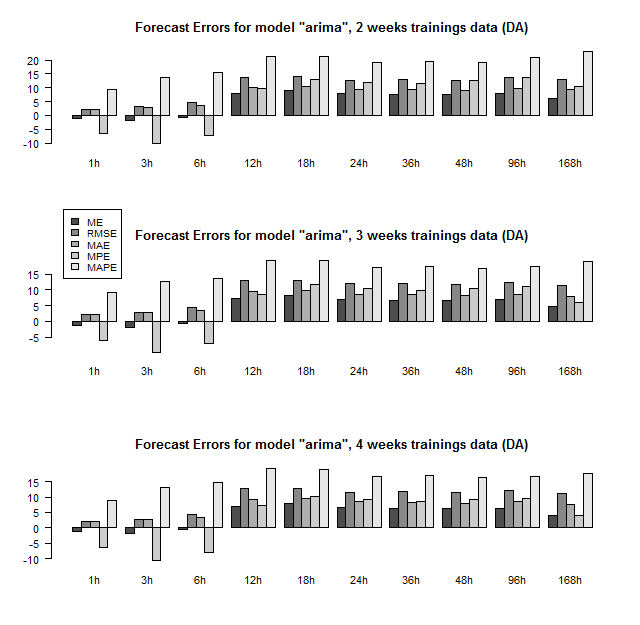
\includegraphics[width=0.85\textwidth]{figures/forecasting/da_sim_1_x_1w_1w_arima.png}
	\caption{Aggregated accuracy measures for ARIMA model and trainings data of 2, 3 and 4 weeks, Nord Pool Spot, Hamina}
	\label{fig:da_sim_1_x_1w_1w_arima}
\end{figure}

\begin{figure}[htbp]
	\centering
		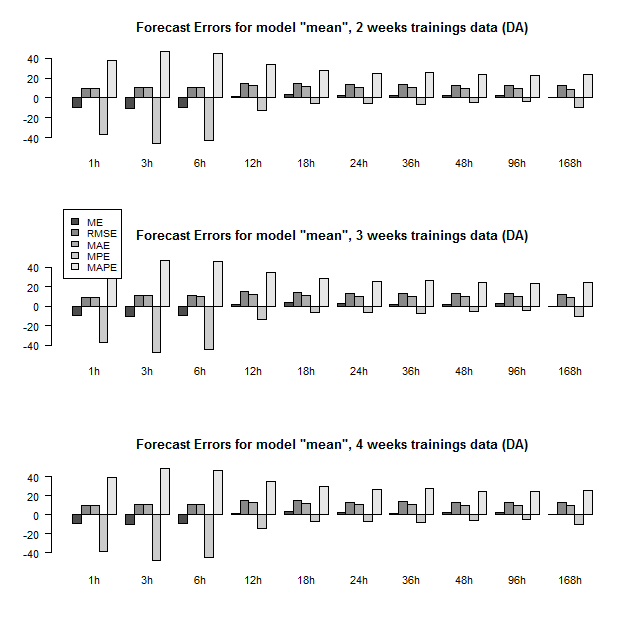
\includegraphics[width=0.85\textwidth]{figures/forecasting/da_sim_1_x_1w_1w_mean.png}
	\caption{Aggregated accuracy measures for Mean model and trainings data of 2, 3 and 4 weeks, Nord Pool Spot, Hamina}
	\label{fig:da_sim_1_x_1w_1w_mean}
\end{figure}


The result tables as well as graphs emphasize the observations made previously about model behavior. 

What can be observed by investigating the large scale forecast evaluation over all locations is that very different behaviors and scales of forecast errors exist for the same model over different locations (i.e.~datasets). An extreme example is the difference in forecast error distributions of the Nord Pool Spot and Belpex energy markets (tables \ref{ssec:app_tables_nord_pool_spot} and \ref{ssec:app_tables_belpex}, graphs \ref{ssec:app_graphs_nord_pool_spot} and \ref{ssec:app_graphs_belpex}). 

However, the seemingly extreme difference in forecast error distribution is mainly caused by exorbitant values of the MPE and MAPE error measures. This may be attributed to the occurrence of many low valued energy prices (close to zero) in the Belpex energy market which causes very high values for these methods. 

When comparing models TBATS, ARIMA followed by Mean and SES forecast models achieve the best results. Remarkably Mean forecasts outperform forecasts of SES models for almost all data sets of day ahead energy markets regarding forecast horizons $>= 12$. This behavior is reversed for real time markets where SES generally provides better performance. 

TBATS models exhibit the least forecast errors when they are able to capture seasonality appropriately. Otherwise these models show exponential growth of forecast errors over all measures. Due to this instability ARIMA models may be preferred as they exhibit stable forecast errors over most data sets and forecast horizons. 

Another note to error distribtions is that for the same forecast model similar patterns can be observed despite differences across energy markets. Concerning different trainings periods it can be observed that for most methods errors decrease with increasing trainings period, i.e.~four weeks of trainings data exhibits the least errors in most cases. 

Also different distributions are apparent for different error measures, e.g.~RMSE tend to increase with increasing forecast horizon whereas percentage errors (MPE and MAPE) tend to hit their lowest values for forecast horizons of 24h to 48h apart from horizons below 12h. 

Concerning the forecast error measures a focus has been laid on evaluating Root Mean Squared Errors (RMSE) since this measure has been proven to provide the most stable results. Percentage error measures such as Mean Percentage Error (MPE) and Mean Absolute Percentage Error (MAPE) tend to become numerically unstable for low values. Difference based measures such as Mean Error (ME) with non-absolute value differences provide little insights to the actual occurred forecast errors as positive and negative values might cancel each other out. 



\subsubsection{Aggregated Results}

Results have been aggregated over all forecast horizons and for each simulation which are shown in Tables \ref{tab:aggregated_results_nord_pool}, \ref{tab:aggregated_results_belpex}, \ref{tab:aggregated_results_isone} and \ref{tab:aggregated_results_pjm}. Best results have been formatted in bold in the tables. 

ARIMA and TBATS models showed superior results over all forecast horizons and training periods. TBATS models show best results when data can be modeled appropriately but exhibit anomalies in other cases. For different training periods a trend can be detected where forecast errors increase with increasing duration of the trainings period. However, ARIMA models show opposite results where forecast errors consistently decrease with increasing trainings period. 


% latex table generated in R 3.1.1 by xtable 1.8-2 package
% Fri Mar 25 19:35:50 2016
\begin{table}[ht]
\centering
\begin{tabular}{rrrrrrr}
  \hline
 & mean & ses & holts & holtwinters & arima & tbats \\ 
  \hline
2 weeks & 12.37 & 11.60 & 62.76 & 73.98 & 10.22 & \textbf{8.21} \\ 
  3 weeks & 12.57 & 11.60 & 62.90 & 75.55 & 9.50 & \textbf{8.57} \\ 
  4 weeks & 12.72 & 11.60 & 63.23 & 85.85 & 9.26 & \textbf{8.43} \\ 
   \hline
\end{tabular}
\caption{Results of evaluation for Hamina, Nord Pool Spot (DA)} 
\label{tab:aggregated_results_nord_pool}
\end{table}
% latex table generated in R 3.1.1 by xtable 1.8-2 package
% Fri Mar 25 19:35:50 2016
\begin{table}[ht]
\centering
\begin{tabular}{rrrrrrr}
  \hline
 & mean & ses & holts & holtwinters & arima & tbats \\ 
  \hline
2 weeks & 15.77 & 15.23 & 127.13 & 186.82 & \textbf{13.49} & 1.27E+50 \\ 
  3 weeks & 16.07 & 15.27 & 128.05 & 190.86 & 12.94 & \textbf{11.61} \\ 
  4 weeks & 16.25 & 15.30 & 127.03 & 186.37 & \textbf{12.87} & 2.49E+36 \\ 
   \hline
\end{tabular}
\caption{Results of evaluation for St.Ghislain, Belpex (DA)}
\label{tab:aggregated_results_belpex}
\end{table}
% latex table generated in R 3.1.1 by xtable 1.8-2 package
% Fri Mar 25 19:35:50 2016
\begin{table}[ht]
\centering
\begin{tabular}{rrrrrrr}
  \hline
 & mean & ses & holts & holtwinters & arima & tbats \\ 
  \hline
2 weeks & 26.42 & 23.61 & 235.84 & 417.39 & \textbf{24.11} & 5.45E+16 \\ 
  3 weeks & 26.36 & 23.56 & 238.92 & 686.95 & \textbf{22.26} & 1.64E+18 \\ 
  4 weeks & 26.84 & 23.32 & 268.10 & 437.85 & \textbf{21.83} & 2.18E+32 \\ 
   \hline
\end{tabular}
\caption{Results of evaluation for Portland, ISO-NE (RT)}
\label{tab:aggregated_results_isone}
\end{table}
% latex table generated in R 3.1.1 by xtable 1.8-2 package
% Fri Mar 25 19:35:50 2016
\begin{table}[ht]
\centering
\begin{tabular}{rrrrrrr}
  \hline
 & mean & ses & holts & holtwinters & arima & tbats \\ 
  \hline
2 weeks & 17.41 & 15.17 & 148.54 & 333.32 & \textbf{15.02} & 7.57E+13 \\ 
  3 weeks & 17.36 & 15.23 & 147.77 & 318.61 & 14.14 & \textbf{ 13.46} \\ 
  4 weeks & 17.34 & 15.29 & 148.67 & 357.82 & \textbf{14.11} & 5.44E+108 \\  
   \hline
\end{tabular}
\caption{Results of evaluation for Richmond, PJM (RT)}
\label{tab:aggregated_results_pjm}
\end{table}



\subsection{Conclusion of results}

From the discussion of the large scale forecast evaluation in the previous section various conclusions may be drawn. 

\paragraph{Model performance}

Concerning model performance ARIMA models showed the best results over different energy markets, trainings periods and forecast horizons. 
They showed consistently low forecast errors and appeared very stable throughout the simulations. Thus among the observed models ARIMA models may be the best choice considering forecast performance and statbility of results. 

\paragraph{Forecast Horizon}

Concerning forecast horizons it has been observed that horizons from 24 hours to 48 hours provide the best results when considering all models and trainings periods. 
For low horizons up to 12 hours different models may be suggested, i.e.~Holts model provide considerably lower forecast errors for forecast windows of 1 and 3 hours. 
For other than very short-term forecasts a forecast window of 24 to 48 hours provides best results. 

\paragraph{Training periods}

Different model training periods provide different results. Forecast errors have been observed to increase with the duration of the trainings period most of the time except for ARIMA models where the opposite behavior has been detected. Thus for ARIMA models a trainings period of 4 weeks is suggested for model generation. 

\paragraph{Forecast error measures}

As discussed before different forecast error methods provide different results for the same dataset. The ME provides an indication of the symmetry of the error distribution but little information about actual forecast performance. The MAE and RMSE provide a way of reliably model forecast errors where they achieve very similar results while the RMSE emphasizes outliers in the data. Percentage error measures have not been found to provide a reliable source of error measurements due to their instability for low values. Thus MAE and RMSE are considered the preferred way of modeling forecast errors. 








%%%%%%%%%%%%%%%%%%%%%%%%%%%%%%%%%%%%%%%%%
\chapter{Methodology}
\label{ch:methodology}
%%%%%%%%%%%%%%%%%%%%%%%%%%%%%%%%%%%%%%%%%



\section{Energy markets}

%Energy markets have emerged steadily from the mid-eighties. 

An outline of a possible implementation of a competitive energy market is depicted in \cite{hogan1993competitive} which is still valid as of today in many respects. A competitive market captures the advantage of market participants being able to actively shaping the clearing price applicable to both producers and consumers in the market. 




\subsection{Types of energy markets}

Two main models exist for the exchange and types of trading of energy prices in power markets which are bilateral trading and electricity pooling, also called loose pool and tight pool models \cite{onaiwu2009does,hogan1997reshaping,barroso2005classification,reston2012short}.

\subsubsection{Loose pool models}

In bilateral trading or loose pool models utility operators (producers) and energy consumers establish bilateral contracts to determine the terms and conditions applied for trading energy \cite{onaiwu2009does,kalverboer2001electricity}. Generators or producers may also buy electricity from other suppliers in case their own electricity generation does not fit current demand. The exact amount, price and time when tradings take place are negotiated on the contract. Since electricity demand may vary from the negotiated terms the resulting imbalances have to be taken care of by the system operator. 

\subsubsection{Tight pool models}

Electricity pooling in tight pool models provide a way for utility operators to offer a certain amount of energy at a set price. Each generator places a bid containing the quantity and expected price \cite{barroso2005classification}. In return consumers place bids on how much they are willing to pay for a given amount of energy. The intersection of the aggregated demand and supply curves defines the energy price for that hour. 

Still customers, brokers and aggregators have the choice to either establish long term contracts of electricity or rely on the short-term market \cite{hogan1997reshaping}.



%Google Search "`loose pool models"'

%See also paper "`Electricity Transmission Pricing and Technology"' and chapter "`Making bilateral competition work"'

%\url{https://books.google.at/books?id=ycLrCAAAQBAJ&pg=PA282&lpg=PA282&dq=Electricity+Transmission+Pricing+and+Technology&source=bl&ots=okH3qUKJwi&sig=MTrGTYJRV5_KmJP9mbdo6GexiPg&hl=de&sa=X&ved=0CDIQ6AEwAmoVChMI3ce_q_XmxgIVBD8UCh1ngQpT#v=onepage&q=Electricity\%20Transmission\%20Pricing\%20and\%20Technology&f=false}


\subsubsection{Day ahead vs real time markets}

Both day ahead and real time markets exist within the scope of a deregulated wholesale power market. As discussed above, electricity pooling is a flexible way of determining energy prices for a short period of time in the future \cite{hogan1997reshaping}. Prices are set based on current demand and supply and are fixed for a particular point in time. This price is then valid for all market participants during that time period. 

In day ahead markets bids are placed for each consecutive hour of the following day. Thus prices are determined on a very short timescale and may exhibit significant volatility. Prices may change substantially from one hour to the next, up to a factor of ten \cite{huisman2007hourly}. Therefore market operators need to apply profound risk management techniques to alleviate such price spikes. 
%it is hard to predict

The real time market on the other hand is used to compensate demand variations during the day which may result in additional changes in energy prices. 
Due to this characteristic the real time market prices exhibit an even greater volatility than those at the day-ahead market whereby the latter is generally used for reference. 

%TODO Explain difference of intraday - real time markets. Same? See \url{http://www.nordpoolspot.com/How-does-it-work/Intraday-market/}. 

% Another resource (intraday market): https://www.next-kraftwerke.de/wissen/strommarkt/intraday-handel

% EPEX Spot - Intraday

%Der Intraday-Handel dient primär dazu, Fehlmengen oder Überschüsse des eigenen Bilanzkreises durch kurzfristige, untertägige Handelsaktivitäten so gering wie möglich zu halten, um den Prognoseverpflichtungen des Bilanzkreisvertrages nachzukommen und etwaige Ausgleichsenergiekosten zu reduzieren. Mit Hinblick auf immer flexibler werdende Anlagen lässt sich der kurzfristige Handel aber auch dafür nutzen, um den Strom von Anlagen kurzfristig bedarfsgerecht – und somit möglichst gewinnbringend und systemstabilisierend – zu produzieren.
%
%Der Intraday-Handel ist insbesondere von Bedeutung, um unvorhersehbare Änderungen in Stromproduktion und -nachfrage über marktliche Mechanismen aufzufangen, bevor der Einsatz von Regelenergie notwendig wird. So kann beispielsweise ein Kraftwerksbetreiber, in dessen Kraftwerk kurzfristig ein Block ausfällt, bei anderen Marktpartnern den seinem Bilanzkreis nun fehlenden Strom einkaufen. Dem Intraday-Handel kommt daher auch in der Direktvermarktung von Erneuerbaren Energien eine Schlüsselrolle zu, etwa wenn kurzfristig angepasste Wetterprognosen ein ungeplantes Mehr oder Weniger an Stromproduktion aus Solar- oder Windkraftanlagen verheißen.

%TODO Compare real time (5 min?) data with hourly day ahead data (graph). Evaluate volatility and maybe also forecasting behavior (this better suits under forecasting menu). 

% Negative Prices

% See https://www.epexspot.com/en/company-info/basics_of_the_power_market/negative_prices


\subsection{Outline of selected energy markets}



\subsubsection{Nord Pool Spot}


The NordPoolSpot market is the most mature power market to date and has been the first energy market that was established in Europe [c]. 

The NordPoolSpot power market consists of four different markets. %(... relevant citations are found below)

% Definition Website

% See http://www.nordpoolspot.com/How-does-it-work/

% THE POWER MARKET, emerging european energy market



As discussed before some markets exhibit strong seasonalities, while others do not. Nord Pool Spot is an example of a power market with obvious seasonalities in the data which can be taken advantage of when creating forecasting models. 

Below two hourly time series from two locations within Nord Pool Spot are displayed that show significant seasonal behavior. 
See figures \ref{fig:hourly_prices_finland} and \ref{fig:hourly_prices_sweden}.

\begin{figure}[!h]
	\centering
		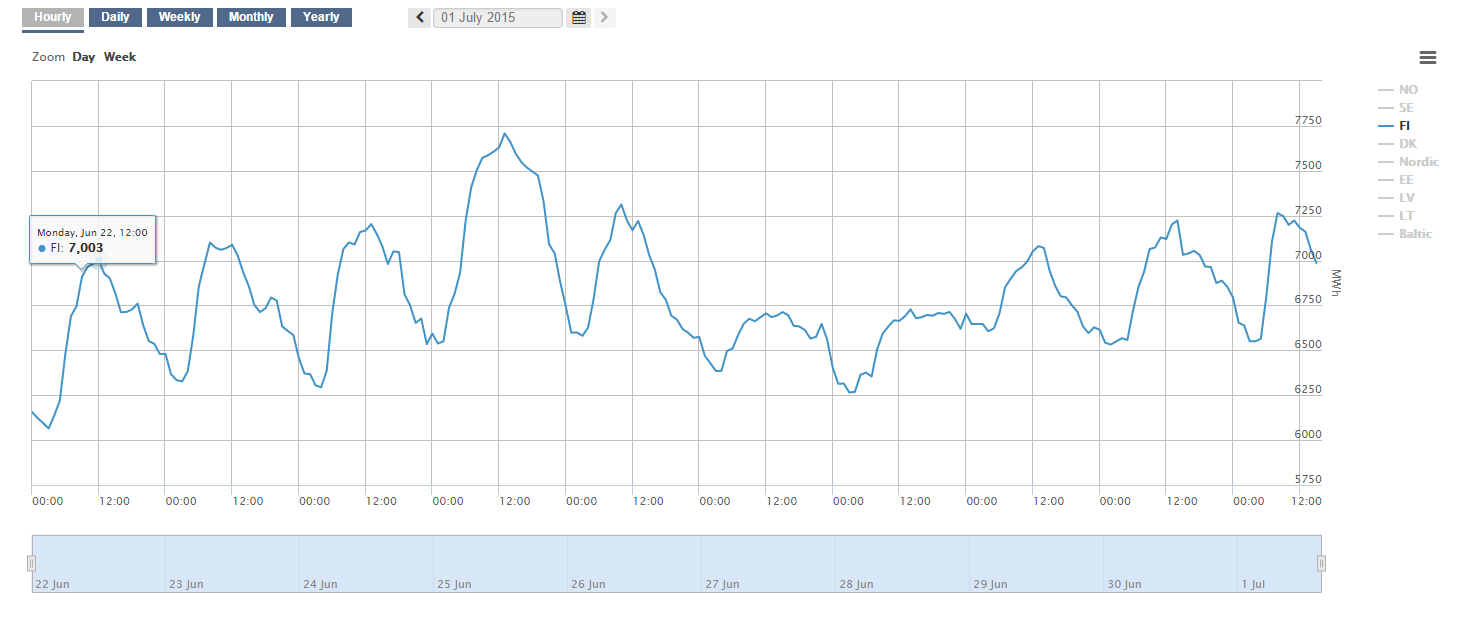
\includegraphics[width=1.00\textwidth]{figures/methodology/hourly_prices_finland.PNG}
	\caption{Finland hourly prices}
	\label{fig:hourly_prices_finland}
\end{figure}

\begin{figure}[!h]
	\centering
		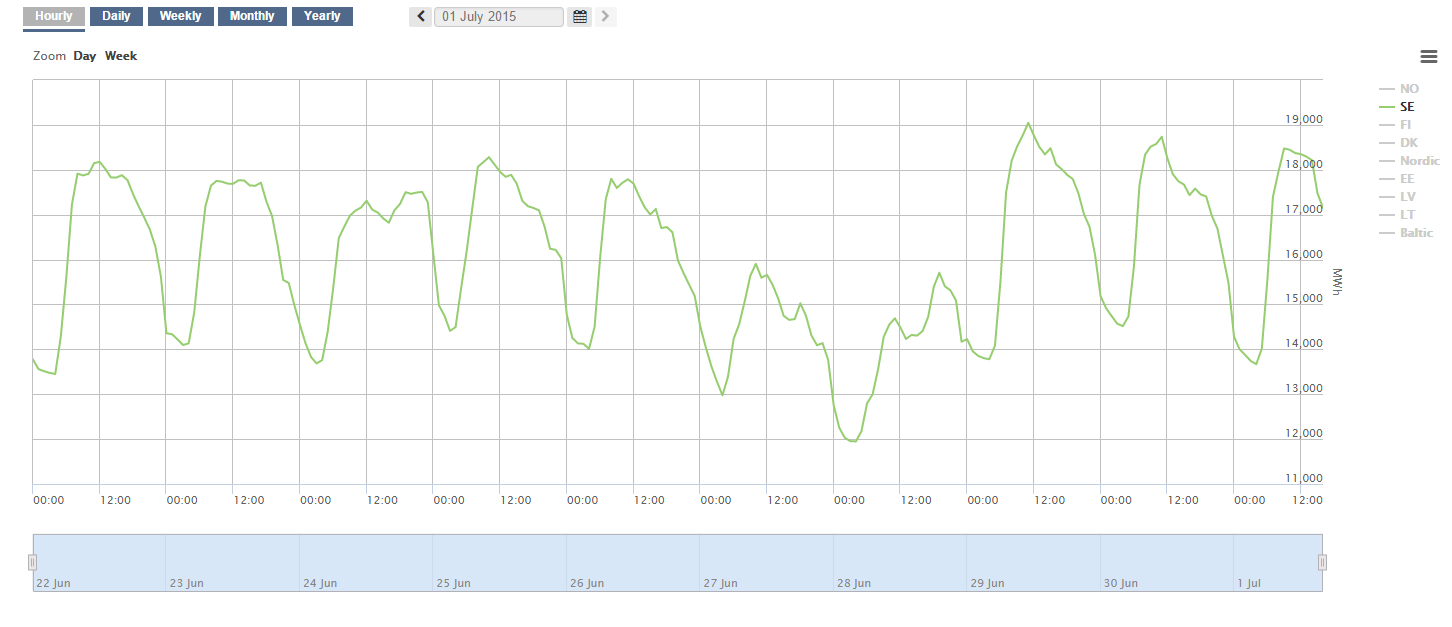
\includegraphics[width=1.00\textwidth]{figures/methodology/hourly_prices_sweden.PNG}
	\caption{Sweden hourly prices}
	\label{fig:hourly_prices_sweden}
\end{figure}




%
%
%[c BEGIN]
%
%\begin{itemize}[-]
%
%\item Financial market (Nasdaq OMX)
%Used for managing risks. Cash settled futures,
%forwards and options. Contracts can be made for
%up to six years. The system price is used as
%reference price.
%
%\item Day-ahead market (Nord Pool Spot)
%Day-ahead auction of power for delivery the next
%day. Nord Pool Spot calculates power prices
%based on supply and demand for every hour the
%following day.
%
%\item Intraday market (Nord Pool Spot)
%Continuous trading up to 30 minutes before
%delivery to adjust power production or
%consumption plans.
%
%\item Balancing market (TSOs)
%Operated by the respective transmission system
%operators. Final adjustments are made to ensure
%the correct frequency in the grid and security of
%supply
%
%\end{itemize}
%
%\emph{The future is Europe}
%
%The future of power trading lies in the
%creation of a single, integrated
%European market and an integrated
%platform.
%This will be the most advanced power
%market yet, offering efficiency in:
%
%\begin{itemize}
%\item Membership
%\item Management of collateral
%\item Cost
%\end{itemize}
%
%[c END] - Nord Pool Spot - Europe's leading power market \url{http://www.nordpoolspot.com/globalassets/download-center/annual-report/nord-pool-spot_europes-leading-power-markets.pdf}




%Nord Pool Spot - Day ahead market
%
%[c BEGIN]
%
%The day-ahead market, Elspot , is the main arena for trading power in the Nordic and Baltic region. Here, contracts are made between seller and buyer for the delivery of power the following day, the price is set and the trade is agreed.
%
%Today there are around 360 buyers and sellers (called members) on Elspot. Most of them trade every day, placing a total of around 2000 orders for power contracts on a daily basis.
%
%\emph{Driven by planning}
%
%Daily trading is driven by the members’ planning. A buyer, typically a utility, needs to assess how much energy (‘volume’) it will need to meet demand the following day, and how much it is willing to pay for this volume, hour by hour. The seller, for example the owner of a hydroelectric power plant, needs to decide how much he can deliver and at what price, hour by hour. These needs are reflected through orders entered by buyers and sellers into the Elspot trading system.
%
%\emph{Setting the price and closing the deal}
%
%12:00 CET is the deadline for submitting bids for power which will be delivered the following day. Elspot feeds the information into a specialist computer system which calculates the price, based on an advanced algorithm. Put simply, the price is set where the curves for sell price and buy price meet.
%
%\emph{Supply and demand}
%
%Hourly prices are typically announced to the market at 12:42 CET or later. Once the market prices have been calculated, trades are settled. From 00:00 CET the next day, power contracts are physically delivered (meaning that the power is provided to the buyer) hour for hour according to the contracts agreed.
%
%\emph{The cost of transmission constraints}
%
%While supply and demand are the key factors determining the hourly market prices, transmission capacity also plays a role. Bottlenecks can occur where power connections are linked to each other, if large volumes need to be transmitted to meet demand. To relieve this congestion, different area prices are introduced. In other words, when transmission capacity gets constrained, the price is raised to reduce demand in the areas affected.
%
%[c END] - Nord pool Spot Elspot Market \url{http://www.nordpoolspot.com/How-does-it-work/Day-ahead-market-Elspot-/}



%Nord Pool Spot - Intraday market
%
%[c BEGIN]
%
%Elbas  is an intraday market for trading power operated by Nord Pool Spot. Covering the Nordic and Baltic region as well as Germany and recently extended to include the UK, Elbas supplements Elspot and helps secure the necessary balance between supply and demand in the power market for Northern Europe.
%
%The majority of the volume handled by Nord Pool Spot is traded on the day-ahead market. For the most part, the balance between supply and demand is secured here. However, incidents may take place between the closing of Elspot at noon CET and delivery the next day. A nuclear power plant may stop operating in Sweden, or strong winds may cause higher power generation than planned at wind turbine plants in Germany. At Elbas, buyers and sellers can trade volumes close to real time to bring the market back in balance.
%
%Trading close to real time
%
%At 14:00 CET, capacities available for Elbas trading are published. Elbas is a continuous market, and trading takes place every day around the clock until one hour before delivery. Prices are set based on a first-come, first-served principle, where best prices come first – highest buy price and lowest sell price.
%
%Increasingly important
%
%The intraday market is becoming increasingly important as more wind power enters the grid. Wind power is unpredictable by nature, and imbalances between day-ahead contracts and produced volume often need to be offset. Elbas will play a key role in the development of intraday power trading in Europe. Future prospects indicate exponential growth, reaching 1.900 GW installed wind capacity worldwide in 2020 (Source: World Wind Energy Association). This type of market can be a key enabler to increase the share of renewable energy in the energy mix. 
%
%[c END] - Nord pool Spot Intraday Market \url{http://www.nordpoolspot.com/How-does-it-work/Intraday-market/}




\subsubsection{ISO New England}

The market of ISO New England offers day ahead as well as real time energy prices where day ahead prices are available at an hourly interval while (preliminary) real time prices are available both at hourly and five minute intervals\footnote{\url{http://www.iso-ne.com/}}. 

Current locational marginal prices (LMPs) can be downloaded from a base url\footnote{\url{http://www.iso-ne.com/static-transform/csv/histRpts/da-lmp/}} and a specialized suffix depending on the file and date (e.g.~WW\_DALMP\_ISO\_20150414.csv). In this case, files are provided in csv format for better machine processing. 

%Example: 
%\begin{verbatim}
	%H,"Date","Hour Ending","Location ID","Location Name","Location Type","Locational Marginal Price",
	%"Energy Component","Congestion Component","Marginal Loss Component"
	%D,"04/14/2015","02","4006",".Z.SEMASS","LOAD ZONE",14.82,14.85,0.01,-0.04
	%D,"04/14/2015","02","4007",".Z.WCMASS","LOAD ZONE",14.94,14.85,0.01,0.08
	%D,"04/14/2015","02","4008",".Z.NEMASSBOST","LOAD ZONE",14.84,14.85,0.01,-0.02
%\end{verbatim}

A summary of all data that is available is provided for day ahead as well as real time prices\footnote{\url{http://www.iso-ne.com/isoexpress/web/reports/pricing/-/tree/zone-info}}. It is described as ``zonal information'' on the website to emphasize the locational character of the prices. 


\subsubsection{EEX}

The European Energy Exchange (EEX) is a power market operating for the market area of France, Germany/Austria and Switzerland. Each of these regions exhibits a separate spot market where prices are traded for the respective country. 
The actual trading takes place on EPEX SPOT, an organisation that drives the integration of power markets in Europe where EEX is a part of. It consists of an intraday (real time) and day ahead market for trading during the day and for the next day, respectively. 

Several info products are available on the market for end-of-day data (EOD) that cover historical as well as current trading data from the spot and derivatives markets. 
Data is available on subscription for all of the above mentioned regions. Available data formats include csv, excel and xml files, provided on demand on a ftp server. 
Depending on the type of product and the time period available different fees apply and have to be paid in advance. 
Access is granted to a vast amount of historical energy price data for the derivatives as well as the spot market for energy and other commodities like natural gas and coal where both prices and trading volumes are included. 

Naming conventions designating the different areas of trading are defined as follows: 

\begin{itemize}

\item \emph{PHELIX} The Physical Electricity Index denotes the area of Germany and Austria

\item \emph{SWISSIX} The Swiss Index denotes the area of Switzerland

\item \emph{FRANCE} The index for France denotes the area of France

\item \emph{ELIX} The European Electricity Index defines prices valid for all of Europe (?)

\end{itemize}


\subsubsection{APG}

Austrian Power Grid\footnote{\url{http://www.apg.at/de/markt/strommarkt}}



\subsubsection{PJM}

See at \url{http://www.pjm.com/}. 


\subsubsection{OMIE - Spanish power market}

OMIE represents the wholesale energy market for the iberian region. \footnote{\url{http://www.omel.com/en/inicio}}

EDP (Energias de Portugal) is an energy company in cooperation with the wholesale electricity market for Spain, Portugal and is also responsible for delivery and transmission of energy to other countries. \footnote{\url{http://www.edp.pt/en/aedp/sectordeenergia/sistemaelectricoespanhol/Pages/SistElectES.aspx}}


\subsubsection{Brazilian power market}

The brazilian power market exhibits special conditions as it is heavily based on hydro power generation \cite{reston2012short}. In this market the tight pool model is applied where generation dispatch is centralized by an Independent System Operator (ISO). 



\subsection{Terms and definitions}

\subsubsection{Definition of 'Clearing Price'}

The following is a definition of clearing price from Investopedia\footnote{\url{http://www.investopedia.com/terms/c/clearingprice.asp}}. 

\begin{quote}
The specified monetary value assigned to a security or asset. This price is determined by the bid and ask process of buyers and sellers interested in trading the security.

In any exchange, sellers prefer to part with their assets for the highest price possible while investors interested in buying the same asset desire the lowest purchase price possible. At some point, a mutually agreeable price is reached between buyers and sellers. It is at this point that economists say the market has "cleared" and transactions take place. Thus, the clearing price of an asset is the price at which it was most recently traded.
\end{quote}



%google Search : "`tight pool models electricity"'
%
%Google Books "`Making Competition Work in Electricity"'
%\url{https://books.google.at/books?id=Pki4tu3P8iIC&pg=PA286\&lpg=PA286\&dq=tight+pool+models+electricity\&source=bl\&ots=drkU0A9H3C\&sig=m_J7JCkGjf5ydml2fdbFQB50ojE\&hl=de\&sa=X\&ved=0CCQQ6AEwAGoVChMIgoLZjffmxgIVTLYUCh3DEQBT#v=onepage\&q=tight\%20pool\%20models\%20electricity\&f=false}
%
%Also see Figure 3.2 in the book on page 43. 
%
%Chapter 4: Requirements for competition- Demand side

The clearing price is set at the intersection of the demand and supply curves, see Figure \ref{fig:market_demand_supply}



\begin{figure}[!h]
	\centering
		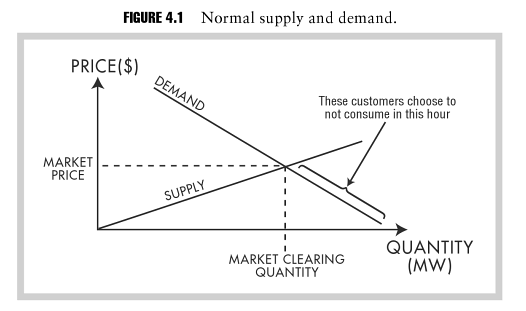
\includegraphics{figures/methodology/market_demand_supply.PNG}
	\caption{Demand Supply Chart}
	\label{fig:market_demand_supply}
\end{figure}



\subsubsection{Locational marginal price}

See definition by ISO-NE\footnote{\url{http://www.iso-ne.com/participate/support/faq/lmp}}. 

%TODO explain LMP (-> see ISO New England energy data, \textbf{smd hourly}!)

\subsubsection{System marginal price (SMP)}

A price type described by \cite{szkuta1999electricity}. 

\subsubsection{System Load}

%TODO

Some energy markets provide the total system load as measured by metering. It is used for day-ahead and long term forecasting purposes and in addition it serves as important indicator in reports. The system load for the ISO New England energy market is calculated by $System Load = generation - pumping + net\_interchange$


\subsubsection{Forward Capacity Market (FCM)} 

A forward capacity market is used to ensure having enough capacity for a specific amount of time into the future. A capacity commitment period (CCP) ensures that a certain amount of capacity will be available during that period. For example, the CCP at ISO-NE is set as one year ranging from June 1st until May 31st. 

The market has to ensure that the \emph{Installed Capacity Requirements (ICR)} for the corresponding region are met. These requirements are defined for each capacity commitment period and define the amount of capacity needed to meet estimated peak and reserve demands. Important measures to define the ICR are the local sourcing requirements (LSR) and maximum capacity limits (MCL) that define the constraints given by market participants. %(QUOTE)In addition the Hydro-Québec Interconnection Capability Credits (HQICCs), are a key input into the calculation of the ICR.

The actual procurement of resources for each capacity commitment period is determined by a \emph{Forward Capacity Auction (FCA)} which aims to meet the defined ICRs for the given period.
This auction is carried out three years ahead of the related CCP to ensure that enough resources will be available during that period. \emph{Reconfiguration Auctions (RA)} are then executed annually until the start of the CCP and continued monthly afterward. During an RA capacity resources may be amended to adapt to potential changes in capacity zones. 

At the FCM of ISO New England there is also the option of making a composite offer where different capacity resources may join their capacity offers (useful i.e.~in case of single season capacities) to result in a single resource offer at the market. 

%Capacity resources <-> energy suppliers/providers?

%See definition at the website of ISO NE\footnote{\url{http://www.iso-ne.com/markets-operations/markets/forward-capacity-market}}.

\subsubsection{Regulation market}

Definition by the ISO NE power market\footnote{\url{http://www.iso-ne.com/markets-operations/markets/regulation-market}}:

\begin{quote}
The Regulation Market is the mechanism for selecting and compensating market participants to provide regulation—the capability of specially equipped generators and other energy sources to increase or decrease output or consumption every four seconds. Participants allow their Automatic Generation Control (AGC) resources to be controlled by the ISO using automated signals to balance both second-by-second variations in demand and the system frequency, which must be kept constant. This market helps ensure that the ISO meets the North American Electric Reliability Corporation Real Power Balancing Control Performance Standard (BAL-001-0). Two regulation clearing prices are calculated: one for capacity and one for actual service mileage.
\end{quote}




\subsubsection{Two settlement system: Day ahead vs Balancing market}

A two settlement system has been defined for the PJM power market (PJM standing for Pennsylvania, Jersey, Maryland)\cite{lambert2001creating}. 

A two-settlement system in power markets is understood as a system comprising a day ahead as well as a real time (balancing) power market\cite{lambert2001creating}. 




\section{Forecasting}

\subsection{Introduction}

Since the occurrence of competitive energy markets forecasting of energy prices has been vital to utility operators. 


\subsection{Forecasting models}

%TODO
Discussion of suitable models for price time series from various energy markets. 


\subsubsection{Random walk}

A random walk model is best suited for series that exhibit major fluctuations on a short term and where no apparent trend can be recognized \cite{makridakisforecasting}(pg. 461). Thus this model can be described by an accumulation of a random error over time (equation \ref{eq:random_walk}). 

\begin{equation}
Y_t = \sum e_t
\label{eq:random_walk}
\end{equation}

$Y_t$ denotes the value of the time series at time point $t$ whereas $e_t$ is a timeseries of random errors where the errors exhibit no correlation and are normally distributed \cite{makridakisforecasting}(pg. 461). 

In \cite{makridakisforecasting}(pg. 464) it is stated that the behavior of economic and business series in particular can be characterized by a random walk model since they show so-called cycles or random fluctuations around a possible trend. 

As it is impossible to accurately predict upcoming values or cycles of a random walk model by definition one of the most suitable prediction models is the ``naive forecast'' where the forecasted value of the upcoming timestamp is set equal to the last observed value (equation \ref{eq:naive_forecast}).

\begin{equation}
\hat{Y}_{t+i} = Y_t
\label{eq:naive_forecast}
\end{equation}



\subsubsection{ARIMA models}

\emph{ARIMA model generation}

See Box-Jenkins Methodology. 


\subsubsection{Neural Network models}

An approach of using artificial neural networks (ANN) as a model to forecast short term electricity prices is presented in \cite{szkuta1999electricity}. 


\paragraph{Competition}

Neural network forecasting competition available from 2008\footnote{\url{http://www.neural-forecasting-competition.com/NN5/}}. 




\subsubsection{Forecasting benchmarks}






\subsection{Accuracy measures}


\subsection{Model selection}



\subsubsection{Autocorrelation}



The autocorrelation function determines the existence or non-existence of correlation between lagged variables within a time series. 

That is, the correlation between a point in the time series to another point in the same time series is calculated where the gap between the two points is fixed by the given lag. 

The autocorrelation is calculated as an autocorrelation coefficient in equation \ref{eq:autocorr_coeff}

\begin{equation}
R_h = \frac{C_h}{C_0}
\label{eq:autocorr_coeff}
\end{equation}


where $C_h$ denotes the autocovariance function and $C_0$ the variance function 
(see equations \ref{eq:autocov_func} and \ref{eq:variance_func}). 


\begin{equation}
C_h = \frac{1}{N} \sum\limits_{t=1}^{N-h} (Y_t - \bar{Y}) (Y_{t+h} - \bar{Y})
\label{eq:autocov_func}
\end{equation}


\begin{equation}
C_0 = \frac{1}{N} \sum\limits_{t=1}^{N} (Y_t - \bar{Y})^2
\label{eq:variance_func}
\end{equation}


Explanation: The autocovariance function determines the (average) covariance between variables with the given lag while the variance function determines the maximum (average) variance over all timestamps (t=1 to N). 


See \url{http://www.itl.nist.gov/div898/handbook/eda/section3/autocopl.htm}


\subsubsection{Box Cox transformation}

The Box Cox transformation is used to transform a series based on a non-normal distribution to a normal distribution. This is done via log and exponential transformations. 

See \url{http://www.isixsigma.com/tools-templates/normality/making-data-normal-using-box-cox-power-transformation/}



\subsection{Energy price related forecasts}



\section{Cloud-based Simulator}


\subsection{Motivation}

\subsection{Structure of simulator}

\subsection{Functional requirements}

%TODO 
Discuss impact of evaluation of bandwidth costs. In \cite{rao2010minimizing} %(page 7) 
bandwidth costs are deliberately neglected, but the option should be still taken into account. As these costs directly relate to costs of migrations it is vital to include and model them within the scenarios. 

\subsection{Non-functional requirements}

\subsection{Incorporating forecast models}

As already discussed in the introduction %TODO WHERE ?(forecast chapter? TODO) 
forecasting is an integral component of the simulation as it should support in decision making when assigning workload and performing migrations. Since forecast errors can have a negative impact on workload allocation which may result in non-optimal workload distributions \cite{de2013study} it is of paramount importance that the forecast models are trained thoroughly and forecast errors are kept at a minimum. In order to reduce the impact of forecast errors in the simulation forecasting is done several hours into the future whereby the results are averaged to obtain a broader estimate of energy prices of the near future. 


\subsection{Simulation runs}



\section{Cost models}

Cost models are required to map the servers' energy consumption to costs depending on current energy prices. Different cost models exist exhibiting higher or lower accuracy and differ in their type of calculation. 

In this thesis several assumptions have been made: 

\begin{itemize}

\item \textbf{idle power.} A server has a defined idle power (e.g.~100 Watts (W)). This is the power that is drawn when the server is in idle mode (no tasks are running). 

\item \textbf{peak power.} A server has a defined peak power (e.g.~200 Watts (W)). This is the power that is drawn when the server runs on maximum load (maximum number of tasks running). 

\item \textbf{utilization.} Each server has a utilization between 0 and 100 percent. A utilization of zero percent means the server is idle, in contrast a utilization of hundred percent means the server is at peak load. 

\item \textbf{power consumption.} The power consumption is defined as the effective power consumed by a server during a certain period of time (e.g.~one hour). The result is a measure of power consumed per time (e.g.~150 Watt hours (Wh) for a server running on 50\% utilization for one hour)\footnote{\url{http://whatis.techtarget.com/definition/kilowatt-hour-kWh}}. %Energy can also be measured in Joule (J) where one Watt (W) equals 1 Joule per second (J/s)\footnote{\url{http://en.wikipedia.org/wiki/Kilowatt_hour}}. Thus one kilowatt hour equals $3.6 * 10^6$ kilojoules. 

\item \textbf{energy price.} The energy price is taken from the energy market that the data center is connected to. These prices typically change every hour which is therefore the relevant time interval for all further operations. 

\end{itemize}

From these assumptions a simple cost model can be derived. Since power is measured per hour in Watts and prices are given per Kilowatt Hours (kWh) the power consumed by servers can be directly mapped to energy costs. This model is simplified in that it does not consider frequency scaling or other power measures taken for a server (suspend, sleep mode). Thus it serves as a base for comparing different scenarios and it is also useful to get a first impression on the overall power consumption and costs involved in a given scenario. 

A cost model is essential for evaluating the usefulness of the approach presented in this thesis as the ultimate goal is to reduce energy related costs of geographically distributed and connected data centers based on changing energy prices. 





%%%%%%%%%%%%%%%%%%%%%%%%%%%%%%%%%%%%%%%%%
\chapter{Results}
\label{ch:results}
%%%%%%%%%%%%%%%%%%%%%%%%%%%%%%%%%%%%%%%%%



\section{Architectural outline}

%\subsection{Application Server}
%
%\subsubsection{Datamanagement}
%
%\subsubsection{Web Services}
%
%\subsubsection{Scheduling}
%
%
%\subsection{R Server}
%
%\subsubsection{Forecast Models}
%
%\subsubsection{Assessment of Forecasts}
%
%\subsubsection{Forecast error evaluation}
%
%
%\subsection{Simulator}
%
%\subsubsection{Basic structure}
%
%\subsubsection{Configuration}
%
%\subsubsection{External interfaces}
%
%\subsubsection{Scheduler}




% Scheduler Types

% Benefits and drawbacks
 
% Settings and configuration



\section{Model selection}


\section{Simulation and Scheduling}


\section{Statistics and Empirical Evaluation}




%%%%%%%%%%%%%%%%%%%%%%%%%%%%%%%%%%%%%%%%%
\chapter{Discussion}
\label{ch:discussion}
%%%%%%%%%%%%%%%%%%%%%%%%%%%%%%%%%%%%%%%%%



\section{Benefits and limitations}



...

As Qureshi et al.~pointed out in \cite{qureshi2009cutting} most companies would need to renegotiate their energy contracts in order to utilize the proposed approach. Companies renting space in co-location facilities usually pay a fixed price for energy rather than directly taking part in the price offers of wholesale markets. 

Demand response programs are a way of further decreasing energy costs as consumers agree on a reduced price in exchange for a reduced load when it is requested by the grid operator\cite{albadi2008summary}. This is certainly interesting for energy elastic distributed systems that are able to shift load to other locations dynamically. 



\section{Comparison of Related Work}


\section{Discussion of open issues}

%%%%%%%%%%%%%%%%%%%%%%%%%%%%%%%%%%%%%%%%%
\chapter{Conclusion}
\label{ch:conclusion}
%%%%%%%%%%%%%%%%%%%%%%%%%%%%%%%%%%%%%%%%%






ARIMA models showed reasonably good performance, in many cases they showed the best results compared to other evaluated models in this work. 







In \cite{de2013study} it is shown that the cost of optimal assignment is further reduced by increasing the number of locations with data centers assigned to different energy markets and/or by increasing the variability of energy prices. 


\section{Benefits and limitations}



...

As Qureshi et al.~pointed out in \cite{qureshi2009cutting} most companies would need to renegotiate their energy contracts in order to utilize the proposed approach. Companies renting space in co-location facilities usually pay a fixed price for energy rather than directly taking part in the price offers of wholesale markets. 

Demand response programs are a way of further decreasing energy costs as consumers agree on a reduced price in exchange for a reduced load when it is requested by the grid operator\cite{albadi2008summary}. This is certainly interesting for energy elastic distributed systems that are able to shift load to other locations dynamically. 






\section{Future Work}


Forecasting models may be improved, or different models may be investigated based on electricity price data. 

Dynamic Regression (DR) and Transfer function (TF) models have been shown to provide a significantly better performance than ARIMA models \cite{aggarwal2009electricity,weron2005forecasting}. This may be due to the additional regressor variables that are considered in multivariate models (DR and TF) in contrast to models based on a single univariate time series (ARIMA). 

In general multivariate models seem to provide better results than univariate models as they are able to include more information into the model generation process \cite{weron2005forecasting}. 


%%%%%%%%%%%%%%%%%%%%%%%%%%%%%%%%%%%%%%%%%
%%% BACKMATTER %%%%%%%%%%%%%%%%%%%%%%%%%%
%%%%%%%%%%%%%%%%%%%%%%%%%%%%%%%%%%%%%%%%%

\appendix

\bibliographystyle{plain}
\bibliography{references}

\end{document}
